\documentclass[PaulGanssle-Thesis.tex]{subfiles}

\begin{document}
\chapter{Magnetometer Design}
\label{magnetometer.design}
\section{Overview}
\label{magnetometer.design.overview}
\begin{wrapfigure}{R}{0.45\tw}
\vspace*{-0.8\lineheight}
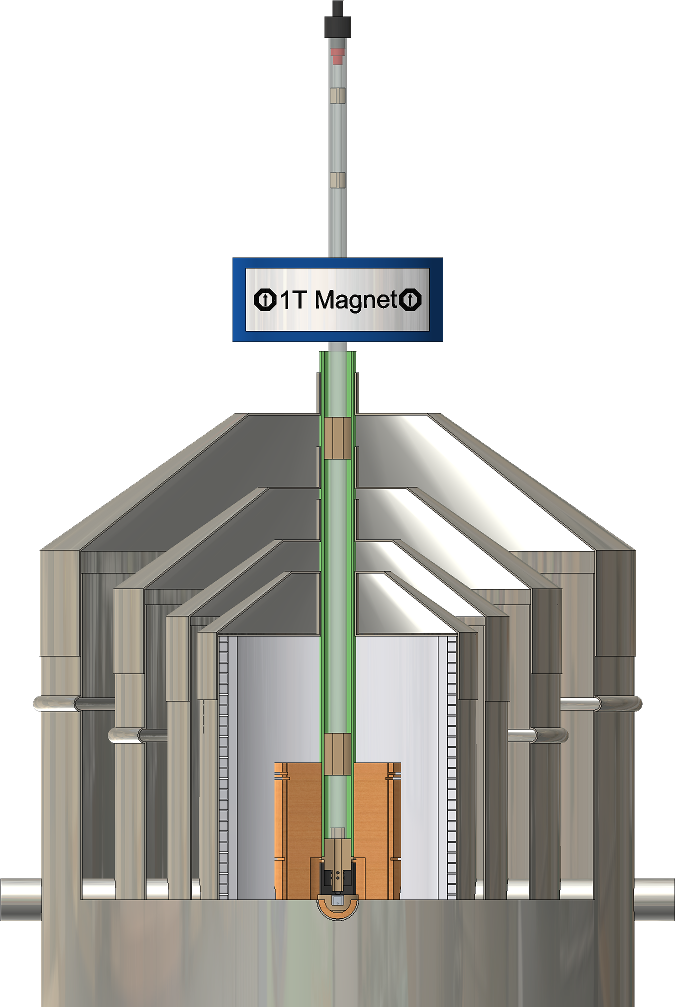
\includegraphics[width=0.45\tw]{figures/magnetometer/MagnetometerCutaway.png}
\caption{A render of our magnetometer.}
\label{fig:MagnetometerCutaway}
\vspace*{-0.8\lineheight}
\end{wrapfigure}

Our magnetometer was designed as a versatile detector for low- and zero-field NMR experiments on relatively small samples. During the course of of the design, two types of cell were used, microfabricated cells provided by the Atomic Devices and Instrumentation group in NIST's Time and Frequency Division, and larger ``cuvette''-style cells purchased frAlso,om Twinleaf Precision Sensors. The magnetometer was configured in a pump-probe configuration (see Sec. \ref{mag.design.pump-probe}) tuned to the D1 resonance of \textsuperscript{87}Rb, operating at zero field in a spin-exchange-relaxation-free (SERF) configuration\cite{Allred2002}. The cells were heated using resistive heating coils wound on ceramic substrates.

The magnetometer used 4 layers of $\mu$-metal shielding using progressive gaps\cite{Dubbers1986} to achieve a total shielding factor of $10^{-6}$. The remaining magnetic field after shielding was removed using a set of three-axis electromagnetic shim coils, the design of which is described in Section \ref{mag.design.shimming}; no gradient shim coils were found to be necessary.

Samples were contained in standard \unit[5]{mm} NMR tubes widely used in high field experiments. The sample spins were pre-polarized\footnote{More on sample polarization in Sec. \ref{nmr.prepolarization}} by pneumatically shuttling the NMR tube between a \unit[1.8]{T} magnet and an air-cooled detection region. NMR pulses and gradients were provided by coils wound on an 3D-printed substrate. surrounding the cell and detector.

\section{Pneumatic Shuttling}
\label{nmr.pneumatic}
\begin{wrapfigure}{r}{0.2\tw}
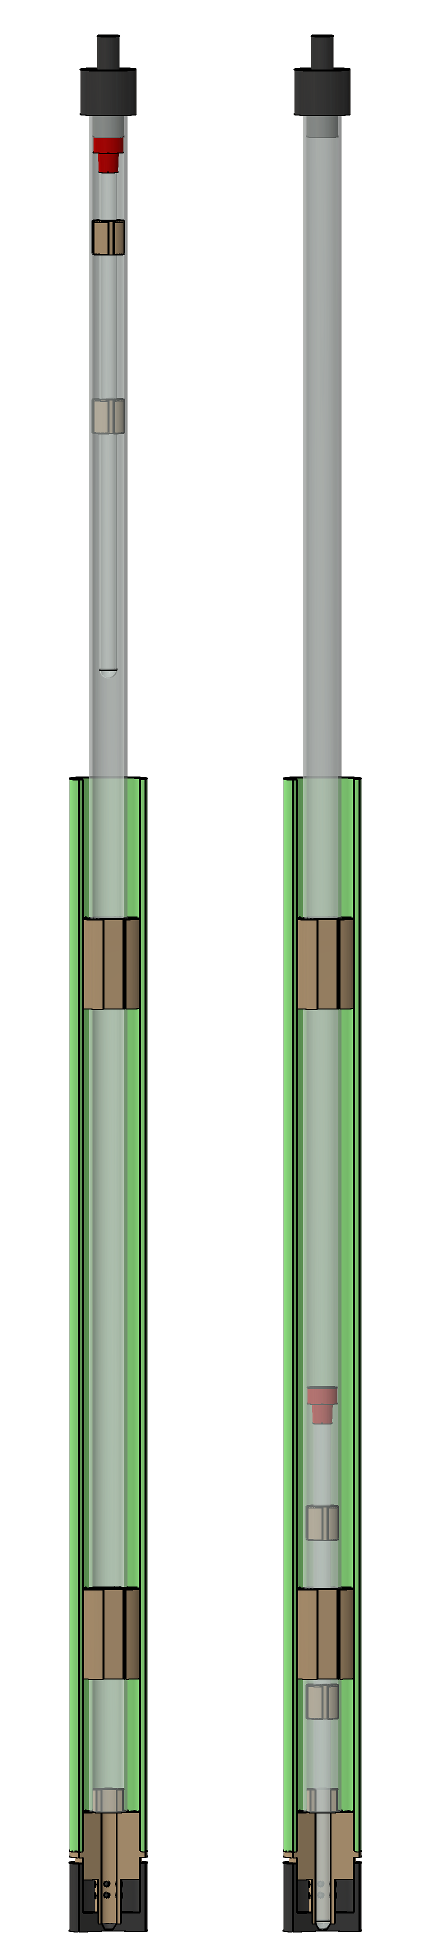
\includegraphics[width=0.2\tw]{figures/magnetometer/FullProbeShuttled.png}
\caption{The sample probe - the sample is pneumatically shuttled between the prepolarizing region and the detection region.}
\label{fig:nmr.probe}
\vspace*{-0.6\lineheight}
\end{wrapfigure}
There are three main ways for a sample to be polarized in a bias field other than the bias field in which the signal is detected. Either a temporary field can be generated during the pre-polarization stage (using an electromagnetic coil or otherwise), a permanent magnet can be temporarily placed in proximity to the sample, or the sample can be temporarily placed in proximity of the permanent magnet. In shielded magnetometers, the application of strong magnetic fields can cause the shields to become magnetized, and as such, the primary method of pre-polarization is by sample shuttling.

In previous magnetometry-based NMR applications, liquid samples have been transferred between polarization and detection regions by pressurized liquid flow between chambers in a cell, driven either by back pressure of gas or using syringe pumps. In these experiments, however, a pneumatic shuttling system has been devised to transfer samples in commercially-available NMR tubes. This has several advantages: it is easier to switch between samples, it can be much faster, it works with non-liquid or extremely viscous samples and often it is much less expensive. The primary disadvantage of the pneumatic sample system is that it is necessary to dissipate much more kinetic energy and design problems can lead to destruction of NMR tubes and --- worse yet --- magnetometer cells. 

For lack of a better word, the sample containment and transfer apparatus is herein called a ``probe'', and the sample reception region is called the ``probe head'', by analogy to the high field probe apparatus. A rendering of the probe components can be found in Fig \ref{fig:nmr.probe}. The outer casing of the probe is \unit[$\frac{1}{16}$]{"} \unit[1]{"} OD G-10 fiberglass, so chosen for its ability to withstand high temperatures. This should be concentric with the pulse coil substrate (see Sec. \ref{nmr.pulsecoil.substrates}) and loose-fitting in the shield access ports (in practice, shield access ports often are not perfectly concentric and parallel tubes, and as such it would be impossible to thread a snug-fitting tube through them). The sample transfer tube is a length of \unit[9]{mm} ID \unit[1]{mm} thickness pyrex glass tubing kept concentric in the outer casing with PEEK tube adapters (see Fig. \ref{fig:nmr.probe.outeradapters}). These spacers are placed $\approx$ \unit[0.5]{"} (\unit[1.27]{cm}) from the bottom of the glass tube and the top of the outer casing, while the glass tube extends beyond the outer casing, long enough that the bottom of a standard \unit[7]{"} NMR tube sits just below the center of the pre-polarizing magnet when the sample is in the pre-polarization position. Between the two spacers is a solenoid wound of \unit[30]{AWG} enamel-coated copper wire, which is used to ensure adiabatic sample transfer (see Sec. \ref{nmr.pneumatic.adiabatic.transfer} below). 


\subsection{Adiabatic Transfer}
\label{nmr.pneumatic.adiabatic.transfer}
\begin{wrapfigure}{L}{0.3\tw}
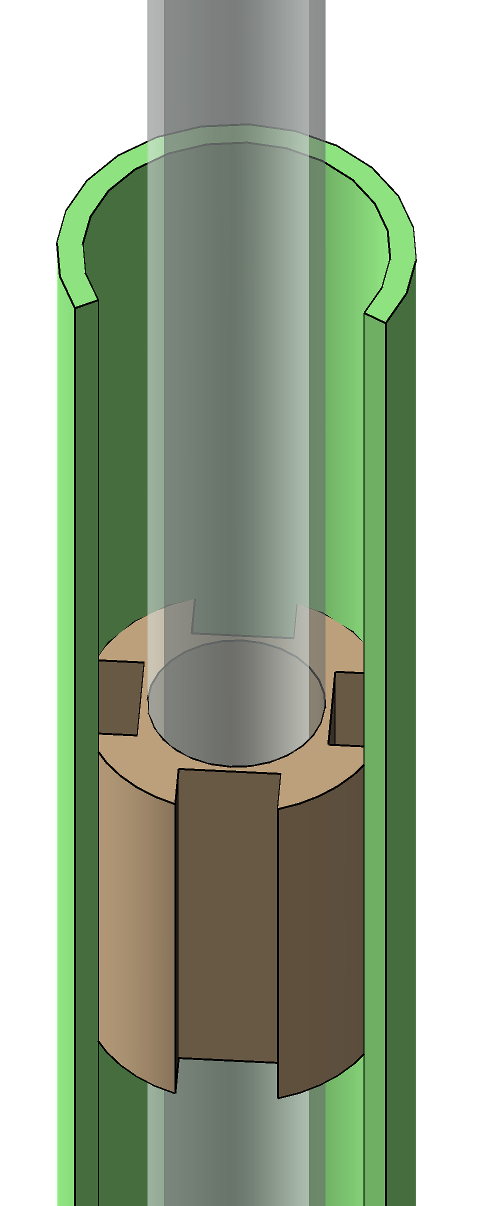
\includegraphics[width=0.3\tw]{figures/magnetometer/TubeSpacerInTube.png}
\caption{Tube diameter adapters used in the probe. The grooves are deep enough to accommodate \unit[$\frac{1}{8}$]{"} tubing used to carry cool nitrogen to the probe head.}
\label{fig:nmr.probe.outeradapters}
\vspace*{-0.5\lineheight}
\end{wrapfigure}
In general, the density matrix of a quantum mechanical ensemble will precess transverse to the direction of the Hamiltonian in the Louisville space representing that Hamiltonian's eigenbasis, with a frequency given by the energy level splitting between the Hamiltonian's eigenstates. This is a more general statement of the principle underlying spin precession transverse to a magnetic field - wherein the eigenstates are aligned parallel and antiparallel with the magnetic field and so the eigenbasis corresponds (to first order) to a physical frame of reference.

When such an ensemble encounters a time-dependent Hamiltonian, the resulting state depends on the rate of the rate of change of the Hamiltonian and the strength of the energy level splitting - when the the rate of change of the Hamiltonian is slow compared to the energy level splittings, the state change is said to occur \textit{adiabatically}, whereas when the Hamiltonian changes quickly with respect to the energy level splittings, the state is said to change \textit{non-adiabatically}. In the non-adiabatic condition (which occurs in NMR experiments when applying pulses), the state of the system is unchanged in response to a sudden change in the Hamiltonian, and if it is not a stationary state of the new Hamiltonian, it will begin to precess in the new Louisville space. In the adiabatic condition, however, precession about the Hamiltonian during periods of incremental change average out over the course of the change in the Hamiltonian, and so the density matrix is ``dragged'' along with the Hamiltonian, maintaining its relative angle in the Louisville space. As a result, stationary states of the initial Hamiltonian will be transformed into stationary states of the final Hamiltonian, and states transverse to the initial Hamiltonian will continue to precess about the final Hamiltonian.

In many cases, the polarization field will not exactly align with either the sensitive direction of the magnetometer or the $z$ direction of the pulsed bias coils. Additionally, as spins are transferred from the polarization to detection region, if they pass through regions in which there is a large gradient (relative to the size of the offset bias field in that location) of fields transverse to the direction of polarization, the spins could decohere during the the sample transfer, killing the signal. Both of these problems are fixed by applying a bias offset field leading from the prepolarization field to the sample detection region which is aligned with the sensitive direction of the magnetometer - this ensures that the Hamiltonian smoothly (and adiabatically) transitions between the polarization and detection regions, and hopefully truncates any small gradients along the way.

In this experimental design, this leading field is provided by a solenoid wound about the inner, glass ``transfer'' tube, and ends several inches above the detection region. The largest practical worry about this is that it might magnetize the shields if the coils are too close and too strong. However, often times the field needs to be \textit{much} stronger directly below the prepolarizing magnet than along the remainder of the path, as the field is shifting rapidly from one on the order of a few Tesla to one on the order of a few Gauss. As a result, in some experiments it is desirable to have both a full leading solenoid which might operate at a few Gauss as well as a larger solenoid positioned further away from the shields but closer to the fringe field of the magnet, which might generate a field of tens to hundreds of Gauss. We have found that for our \unit[2]{T} setup, this does not contribute significantly to the adiabatic transfer and it has been removed, but the necessity of this step is highly dependent on transfer speed and setup geometry and so no general recommendation either way can be made.

To ensure that, in the end, the field is at least aligned exactly with the bias field coils (which are geometrically constrained to be orthogonal to the $x$ and $y$ directions), the bias field coil is also energized during the transfer. This also helps to ensure the homogeneity of the field as the sample travels through the fringe of the solenoid - which is several inches from the cell, both for practical reasons and to reduce magnetic field noise associated with the leading coil.

\subsection{Probe Head Design}
\label{Section:Pneumatic-Shuttling-Probe-Head-Design}
\begin{wrapfigure}{L}{0.25\tw}
\vspace*{-0.75\lineheight}
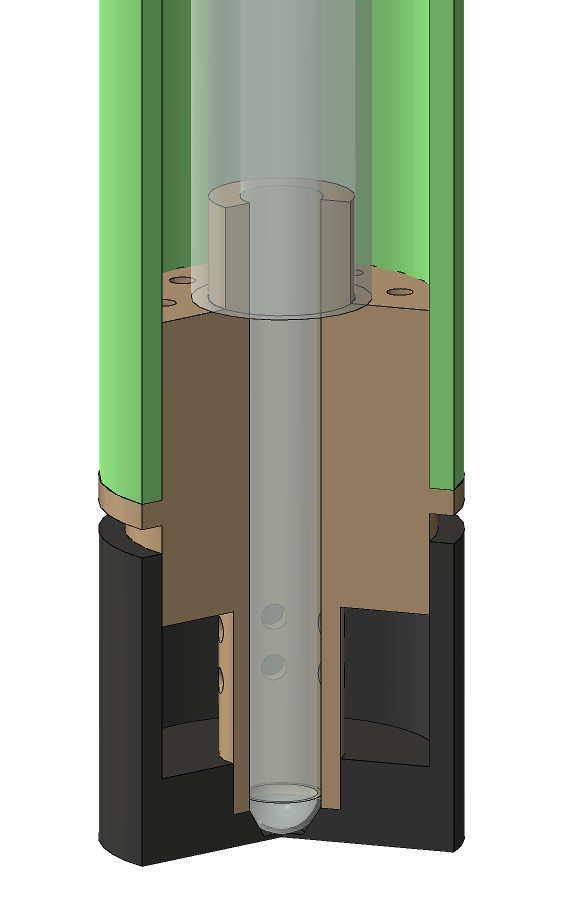
\includegraphics[width=0.25\tw]{figures/magnetometer/ProbeHeadCloseup.png}
\caption{The probe head is designed for thermal insulation and minimization of physical shock.}
\label{fig:ProbeHeadRender}
\vspace*{-0.5\lineheight}
\end{wrapfigure}
The probe head (Fig. \ref{fig:ProbeHeadRender}) has two primary design goals: to thermally insulate the sample from the cell and to protect the sample and the cell from a high-speed collision during sample shuttling. Thermal insulation is necessary because the cell runs at an elevated temperature, a side effect of which is that the inside of the magnetometer reaches thermal equilibrium at some significantly elevated temperature (on the order of \unit[60-100]{\degsym C} depending on cell temperature, air flow, etc), which could have a deleterious effect on the sample, or otherwise interfere with desired measurements. The probe head thermally isolates the samples both to minimize the impact of the elevated temperature in the detection and to allow for the use of cool, dry nitrogen flow to cool the sample without causing undue temperature gradients very close to the cell.

The probe head is divided into two parts - the probe head cap and the main body, both PEEK pieces which are designed to ``slip-fit'' together sufficiently tightly that an airtight seal is formed. Because both pneumatic shuttling and sample cooling (more on which in Sec \ref{nmr.pneumatic.sample}) cause gusts of wind which introduce significant noise into the system, it is important to ensure that the probe head is well-sealed from the detection region.  Generally slip-fit designs can form seals sufficient to this goal because the high-temperature operating environment cause thermal expansion of the components, forming tighter seals than might be possible with room-temperature tolerances. In lower-temperature magnetometers, such as Cs-vapor cell magnetometers, it might be advisable to switch to a system using O-rings or rubber gaskets to prevent leaks into the detection region.

\begin{wrapfigure}{R}{0.4\tw}
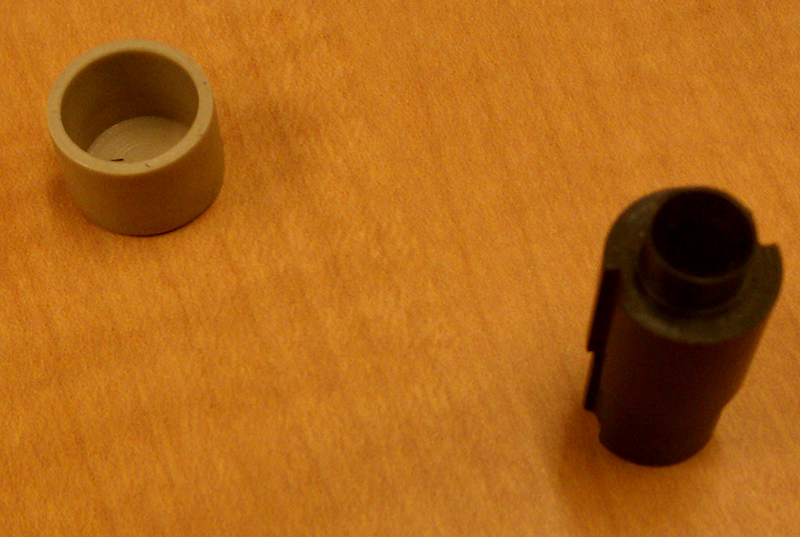
\includegraphics[width=0.4\tw]{figures/magnetometer/ProbeHeadOldCap-Smaller.png}
\caption{An older version of the probe head, with a flat-bottomed cap.}
\label{fig:OldProbeCap}
\vspace*{-0.5\lineheight}
\end{wrapfigure}

The probe head cap is \unit[0.75]{"} (\unit[1.905]{cm}) long with an outer diameter set to just below the outer diameter of the outer G-10 probe casing and an inner diameter set such that it will slip-fit over the probe head body. A square-bottomed hole is milled or lathed out of the center to a depth sufficient to attach solidly to the probe head body while still leaving room for a hollow chamber through which air can flow over the sample for cooling, while also leaving enough thickness at the bottom of the cap to insulate the probe head well from the cell heater. Generally \unit[0.25]{"} (\unit[0.635]{cm}) is chosen for this value. Greater thickness along the bottom of the cap allows for greater thermal insulation and ability to absorb kinetic energy from dropped samples, but may contribute to a larger thermal gradient across the sample - which can give rise to convection. 

\begin{wrapfigure}{L}{0.25\tw}
\vspace*{-0.5\lineheight}
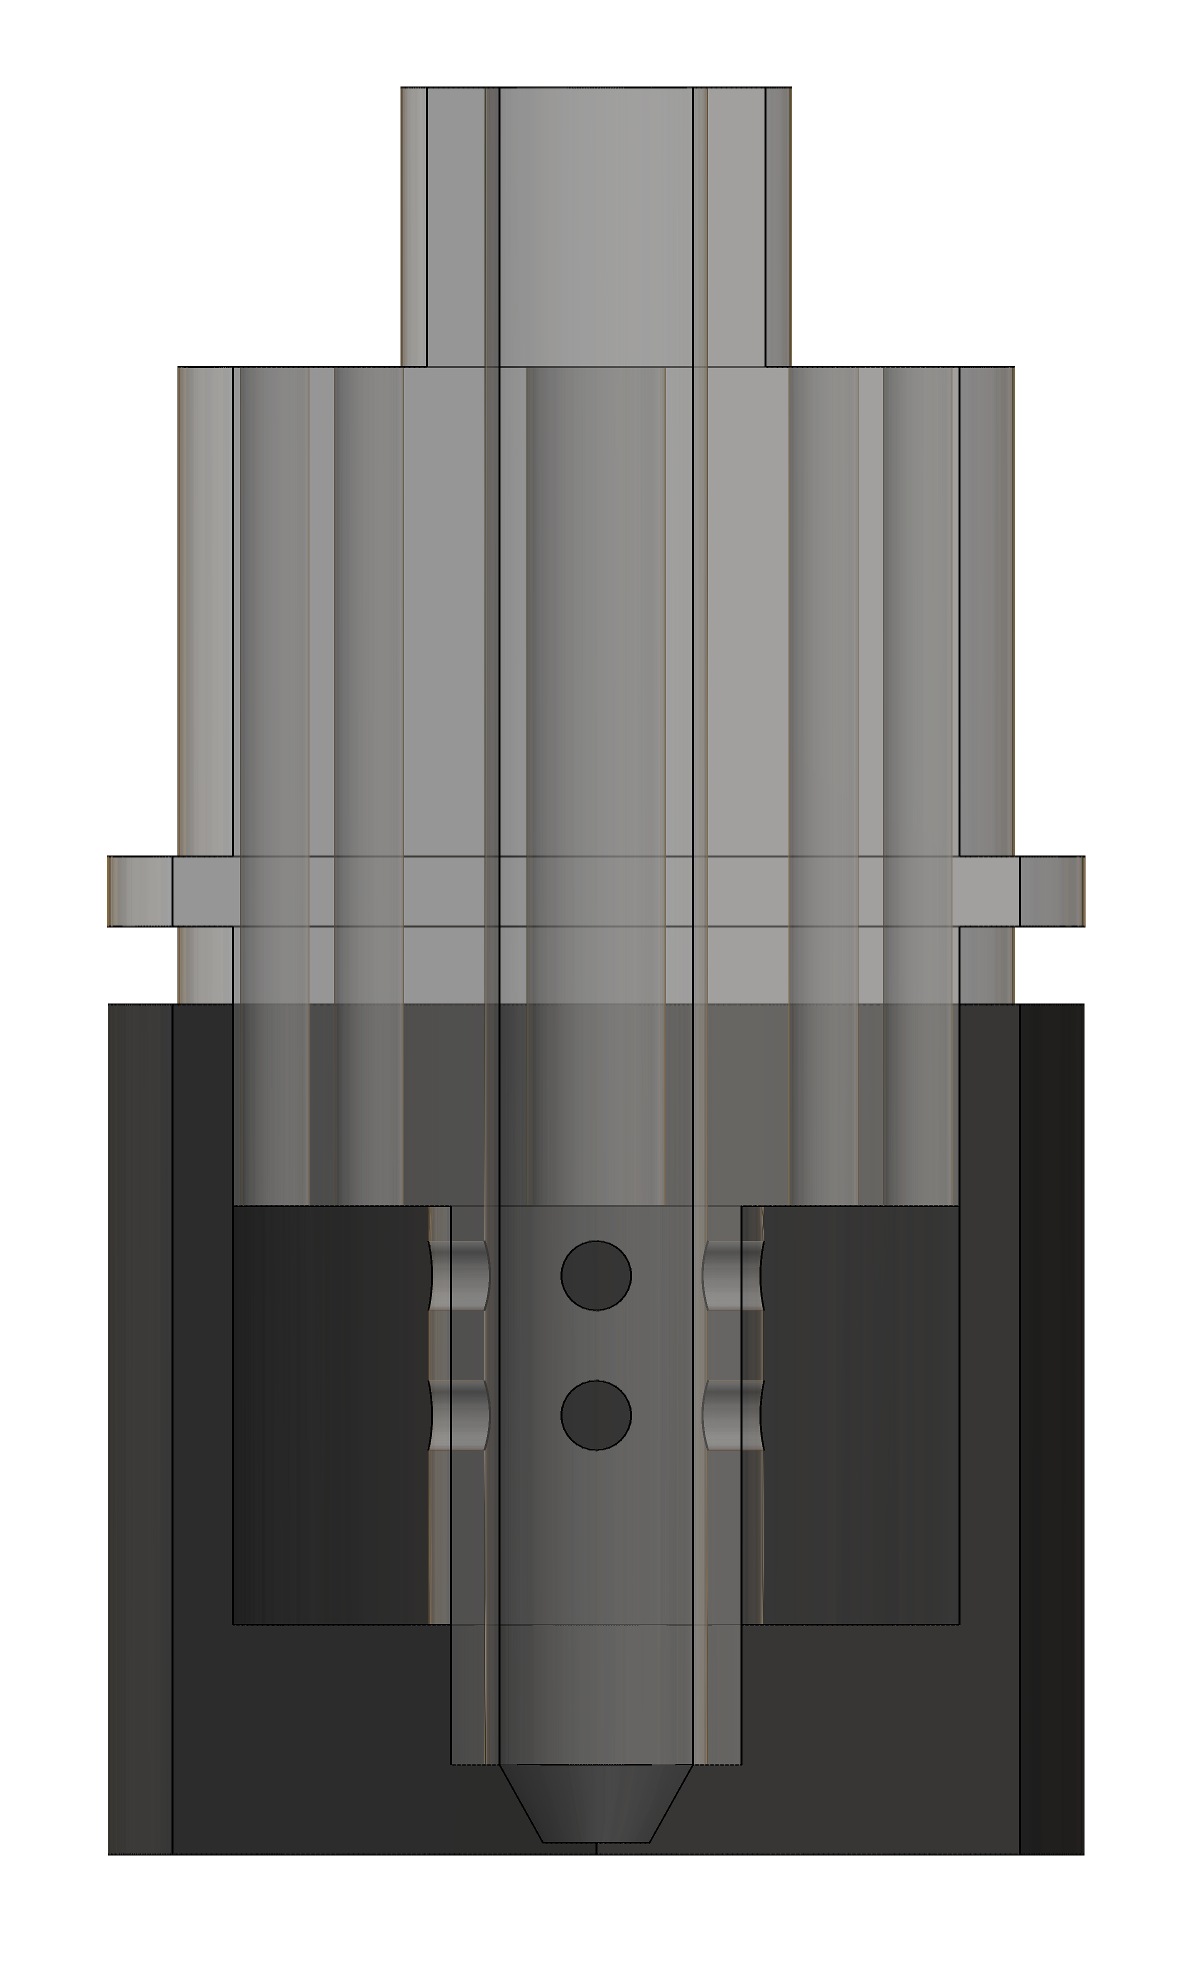
\includegraphics[width=0.25\tw]{figures/magnetometer/ProbeCap.png}
\caption{A render of the new probe head cap, with a tapered cap bottom.}
\label{fig:ProbeCapRender}
\vspace*{-0.5\lineheight}
\end{wrapfigure}

A smaller hole is then milled out of the center of this cap with a diameter sufficient to accommodate the sample transfer tube extruding from the bottom of the probe head body, and milled sufficiently thin that the bottom of the sample sits no more than $\approx$ \unit[100-500]{$\mu m$} from the bottom of the cap. Because the magnetic field generated by the sample dies off proportional to $\sfrac{1}{r^3}$ (where $r$ is the distance between the sample and the sensitive magnetometer volume), it is extremely desirable to minimize the thickness of this landing spot as much as possible without significantly compromising the thermal insulation or the physical protection afforded by the probe head.

In an earlier version of the probe head cap, this landing spot was a \unit[100-200]{$\mu m$}-thick flat panel, which eventually lead to the destruction of at least two magnetometer cells. Although the probe head does not sit directly on the cells (it sits several hundred $\mu m$ above, on small PEEK spacers), the flat-bottomed design does not provide sufficient strength to absorb the kinetic energy of a dropped sample without deformation. In the earliest versions of the probe head cap, samples were able to cause this panel to break off (and the sample to crash through, thus destroying the cell). In later versions, the sample caused this flat region to ``bow out'', allowing the sample to come into contact with the cell. In the current version, however, this problem is solved by using a ball-end mill to match the contours of this ``landing spot'' with the contours of an NMR sample tube. This adds strength and thermal insulation to the cap without compromising on distance, as the sample can only sit such that the bottom part is touching the cap, and so by keeping the nadir of the landing region at \unit[100-200]{$\mu m$} thick and following the contours of the NMR sample tube, the total distance is unchanged.

\label{mag.design.probe.head.body}
\begin{wrapfigure}{r}{0.33\tw}
\vspace*{-0.3\lineheight}
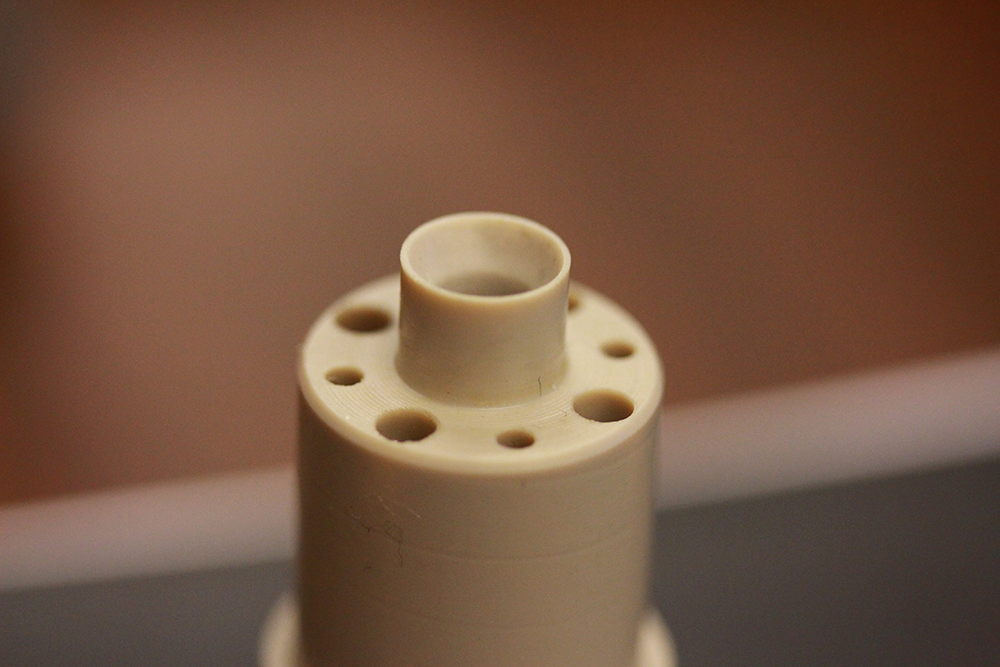
\includegraphics[width=0.33\tw]{figures/magnetometer/NewProbeHeadChamferSmaller.png}
\caption{The top of the probe head is chamfered to prevent falling NMR tubes from landing askew or breaking.}
\label{fig:ProbeHeadChamfer}
\vspace*{-0.5\lineheight}
\end{wrapfigure}
The probe head body is designed to adapt between the glass sample transfer tube, the G-10 casing and the probe head cap, and to allow a strong flow of cooling and shuttling gases through the system. As with the junction between the cap and body, the junction between the probe head body and outer probe casing must be airtight to prevent noise in the sensor region, and as before this is achieved fairly easily with a slip-fit design at elevated temperature. Running through the center of the probe head body is a through-hole with diameter $\lessapprox$ \unit[0.217]{"} (\unit[5.5]{mm}), intended to allow \unit[5]{mm} NMR sample tubes to pass unimpeded. The hole is flat on the bottom, but has a roughly \unit[30]{\degsym} chamfer on top, which allows slightly mis-aligned samples coming in to both smoothly become re-centered in the guidance tube, and to lose some of their kinetic energy prior to hitting the bottom, possibly making for a more gentle and elastic collision at its eventual destination (as it happens, properly made spacers will likely prevent much contact with the side-walls of the probe head, and so in order to take advantage of these collisions, it might be preferable to use looser fit spacers and a narrower channel in the probe head body).

\begin{wrapfigure}{l}{0.35\tw}
\centering
\vspace*{-0.5\lineheight}
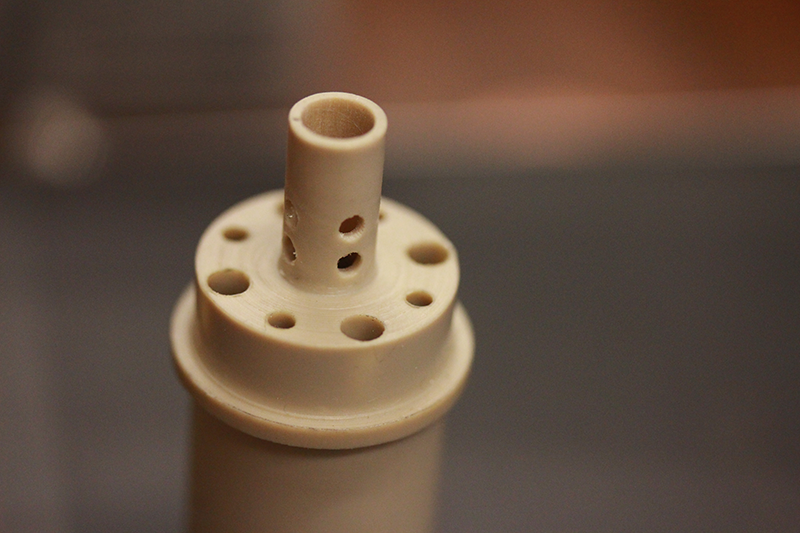
\includegraphics[width=0.35\tw]{figures/magnetometer/NewProbeHeadBottomVentsSmaller.png}
\caption{Vents are placed in the bottom of the probe head to allow air displaced by the falling sample tube to escape rapidly; without these, air is compressed below the NMR tube, slowing or stopping entirely its descent before it reaches the measurement region.}
\label{fig:ProbeHeadVents}
\vspace*{-0.5\lineheight}
\end{wrapfigure}

At the bottom of the probe head body is a \unit[0.3]{"} diameter, \unit[0.5]{"} extrusion which is loose to slip fit in the landing channel of the probe head cap (no seal is necessary or possibly even desirable, but a tighter fit tends to force the two to remain concentrically aligned). Eight \unit[$\sfrac{1}{16}$]{"} holes are drilled high enough that, when the probe head is assembled, they will all be exposed to the hollow sample chamber. These act as vents to allow the cooling air to flow over the summer, and to allow the air under the falling sample to be pushed out of the main body of the probe. At the top of the probe is a \unit[0.25]{"} extrusion with \unit[0.35]{"} (\unit[8.89]{mm}) diameter - this should fit loosely into the glass sample transfer tube, but not slip-fit; because the sample transfer tube has brittle ends, a tight fit is likely to result in the ends of the glass tubes becoming broken either due to minor mis-alignment between the glass tube and the outer casing or thermal expansion of the materials.

Drilled longitudinally through the main body of the probe head body are eight radially distributed holes, six \unit[$\sfrac{1}{16}$]{"} diameter and two \unit[$\sfrac{1}{8}$]{"} holes. The \unit[$\sfrac{1}{16}$]{"} holes serve as vents from the hollow sample chamber, allowing air to flow through the system. The \unit[$\sfrac{1}{8}$]{"} holes are designed to accommodate \unit[$\sfrac{1}{8}$]{"} OD tubing, which brings in the cool, dry nitrogen for sample cooling. Depending on the need for flow, either one or two tubes can be used for this purpose.

The air pumped into the probe head can escape from two channels - either it can escape out of the vents into the probe body or it can push past the sample and escape out the sample tube, which generally buffets the sample tube upwards. We can take advantage of this for sample shuttling by blocking the open end of the probe body and sealing it with parafilm, preventing any air from escaping from the probe body. Vent holes are then drilled into the probe body above the level of the outermost shield, but before the end of the probe - where the vents are most accessible. These vents can then be covered to prevent air from escaping from the probe body, or uncovered to prevent air from buffeting the sample. This is particularly useful when changing samples, as this cannot be done with the pneumatically actuated vacuum in place. Without pushing the sample out with a back-pressure of nitrogen in this way, removing the vacuum source from the transfer tube will cause the sample to drop. It is also not desirable to leave the probe out-flow blocked at all times, as this will cause samples to move during the experiments, leading to noise and uncertainty.

\subsection{Active Sample Cooling}
\label{nmr.pneumatic.sample}
When using cooling nitrogen (which is often at or slightly below room temperature), the sample will soon reach an equilibrium temperature which depends on the temperature of the cell, the equilibrium temperature of the sensitive region of the magnetometer, the nitrogen flow and the exact geometry of the probe head, among other things. However, often this equilibrium temperature will still be slightly above room temperature, and it certainly not be lower than room temperature. When experiments require a sample to be measured at a specific temperature, it is necessary to use a more active cooling approach.

Aiming for greater temperature control, we introduced a liquid nitrogen cooled coil into the cooling line, to start the nitrogen at a significantly lower temperature. After leaving the liquid nitrogen cooling line, the delivery line is wound with a resistive heater attached to a thermocouple, allowing more heat to be added back in as needed. This system is somewhat wasteful, however, and it might be preferable to replace it with a temperature-controlled oil or water bath with a cooling unit. The main concern with most cooling apparatus is that they may introduce some vibrations into the experiment, and so it is important to keep them vibrationally isolated - this is also the case with liquid nitrogen cooling, where the LN2 boil-off can be quite volatile. In our experiments, a dewar was placed on vibration-damping foam, which seemed to remove most if not all of the vibrational noise from boil-off.

Our experiments in this front were not particularly successful, and as they were not particularly necessary to any one project, they were abandoned after early failures. The primary issues encountered were slow response times (it took quite a while for the system to come into equilibrium after each change, and often the LN2 would boil off quickly on this time scale) and sensitive calibration. Without very dry liquid nitrogen, water and (to some extent liquid oxygen) condenses in the lines, preventing any cooling whatsoever. Even then, leaks can develop as plastic tubes and junctions contract in response to low temperatures --- this can introduce some moisture and again cause plugs to form. Finally, when all these practical issues are addressed, often times our samples would freeze in place, cracking the sample tubes and preventing their removal from the probe head (which also tends to contract, making it more difficult for samples to reach the landing spot).

In future cooling system designs, we would recommend the use of a long copper or aluminum wound coil of tubing in a refrigerated bath (a saltwater bath is likely sufficient). This will not help with the slow response times, but it will prevent coolant boil-off from limiting the long-term use of the system. Additionally, either evacuating or strongly insulating all the lines carrying the cooling air is ideal, as significant condensation has been observed when using liquid nitrogen cooling. Finally, the use of cooled nitrogen gas could very well lead the probe head body and cap to contract and break their airtight seal, leading to noise in the magnetometer. In future designs for active cooling, it is likely that the use of low-temperature O-rings or gaskets would be advisable to maintain all seals. This is especially important as sudden temperature shifts at the point of the cell itself can cause immense strain and if any cold liquid were to drip onto the cell (such as condensation on the outside of the probe head cap), the cell would likely be destroyed.

\section{Pulse Coil Design}
\label{nmr.pulsecoil}
\subsection{NMR Pulses}
Most if not all NMR experiments involve the application of sudden, non-adiabatic on-resonance pulses for control of spins. When a field orthogonal to the direction of spin polarization is turned on non-adiabatically, this induces a precession of frequency $\omega_1 = \gamma\mathbf{B_1}$ where $\mathbf{B_1}$ is the amplitude of the applied field. This fact can be used to control spin evolution using pulsed magnetic fields - for example, spins aligned along $z$ can be made to align along $y$ by applying a pulse along $x$ for $t_{\sfrac{\pi}{2}} = \sfrac{\pi}{2\gamma B_1}$\footnote{Here $\gamma$ is in units of angular frequency per magnetic field (\unitfrac{rad$\cdot$Hz}{G}, \unitfrac{rad$\cdot$MHz}{T}, etc). For $\bar{\gamma} = \sfrac{\gamma}{2\pi}$ in units of angular frequency (\unitfrac{Hz}{G}, \unitfrac{MHz}{T}, etc), the value is $t_{\sfrac{\pi}{2}} = \sfrac{1}{4\bar{\gamma} B_1}$}. In a more general form, the tip angle from applying a (possibly time-dependent) magnetic field with amplitude $B_1(t)$ transverse to the spins is given by the integral of the precession during the pulse:

\begin{equation}
\label{eqn:SpinTipAngle}
\theta_p = \int_0^{t_p}\!\gamma B_1(t)t\textrm{d}t
\end{equation}

For a stationary pulse applied to spins at zero field, $B_1$ is constant, and so $\theta_p = \gamma B_1 t$, but in the presence of a bias offset field $B_0 \gg B_1$ along $\vec{\mathbf{z}}$, spins tipped transverse to the field will precess at frequency $\omega_0$, and so the transverse amplitude varies as a function of time. The natural coordinate system for analyzing the spin evolution of such a system is not the laboratory frame but a rotating frame of reference in which unperturbed spins are stationary. This can be achieved by defining time-dependent axes $\vec{\mathbf{x'}}$ and $\vec{\mathbf{y'}}$:

\begin{align}
\label{eqn:RotatingFrameXAxis}
\vec{\mathbf{x'}} & =  \vec{\mathbf{x}}\cos\left(-\omega_0 t\right) - \vec{\mathbf{y}}\sin\left(-\omega_0 t\right) \\
\label{eqn:RotatingFrameYAxis}
\vec{\mathbf{y'}} & =  \vec{\mathbf{x}}\sin\left(-\omega_0 t\right) + \vec{\mathbf{y}}\cos\left(-\omega_0 t\right)
\end{align}

In the lab frame, a static pulse along $\vec{\mathbf{x}}$ is described by Eqn \ref{eqn:StaticFieldXLabFrame}
\begin{equation}
\label{eqn:StaticFieldXLabFrame}
B_x(t) = B_{1}\vec{\mathbf{x}}
\end{equation}

However, when transformed into the rotating frame, the same field is described by Eqn \ref{eqn:StaticFieldXRotatingFrame}:

\begin{equation}
\label{eqn:StaticFieldXRotatingFrame}
B_x(t) = B_{1}\left[\vec{\mathbf{x'}}\cos\left(\omega_0 t\right) - \vec{\mathbf{y'}}\sin\left(\omega_0 t\right)\right]
\end{equation}

So for spins along $\vec{\mathbf{y'}}$, applying the pulse $B_x(t)$ gives a tip angle given by the integral of the amplitude along the transverse $\vec{\mathbf{x'}}$ direction (Eqn \ref{eqn:StaticXPulseOnYPrime}):

\begin{equation}
\label{eqn:StaticXPulseOnYPrime}
\theta_p = \gamma B_{1}\int_0^{t_p}\!\cos\left(\omega_0 t\right)\mathrm{d}t
\end{equation}

For $\omega_0 \gg t_p$, this integral evaluates to 0, and so such a pulse would yield no net tip of the spins. Modulating $B_1$ at frequency $\omega_0$, however, gives a tip angle:

\begin{equation}
\label{eqn:ResonantPulseXPrime}
\theta_p = \gamma B_{1} \int_0^{t_p}\!\cos\left(\omega_0 t\right)^2\mathrm{d}t
\end{equation}

And for $\omega_0 \gg t_p$ this evaluates to $\frac{1}{2}\gamma B_1 t_p$.

\subsection{DC Pulsing}
\label{nmr.pulsecoil.DC}
Our experiments all take place at zero magnetic field. This is a special case of the rotating frame where $\omega_0 = 0$, and so DC pulses can be used for spin manipulation. Because the spins do not precess with respect to the pulse coils, the rotating-frame pulse ``phase'' is replaced with a physical, lab-frame, direction, and as such separate orthogonal coils must be used for pulse application. However, because a DC pulse at zero field is effectively a full quadrature pulse (whereas a single coil in a rotating frame only applies half the quadrature pulse), the tip angle at zero field is twice what it would be for the same amplitude in the RF context. This has consequences for device voltage, as the RF transmitter power is proportional to the waveform root-mean-squared, while the DC power is proportional directly to the amplitude - as such to apply RF pulses of the same power as a DC pulse requires voltage to be stepped up by a factor of $\sqrt{2}$.

\subsection{Coil Designs}
\label{nmr.pulsecoil.designs}
Two sets of pulse coil designs have been used in these experiments - a smaller set of 3 coils wound about a Macor substrate, and a larger set of 4 coils wound about a 3D printed epoxy-infused plaster substrate. In both cases, \unit[30]{AWG} high-temperature magnet wires were wound in grooves machined (or printed) into cylindrical substrates. In the smaller coils, saddle coils are wound about $x$ and $y$ with a Helmholtz pair about $z$. In the larger coils, a ``$g$'' (gradient) coil is wound as an anti-Helmholtz pair.

\begin{figure}[t!] 
\centering
\begin{subfigure}[h]{0.3\tw}
\begin{tabular}{c}
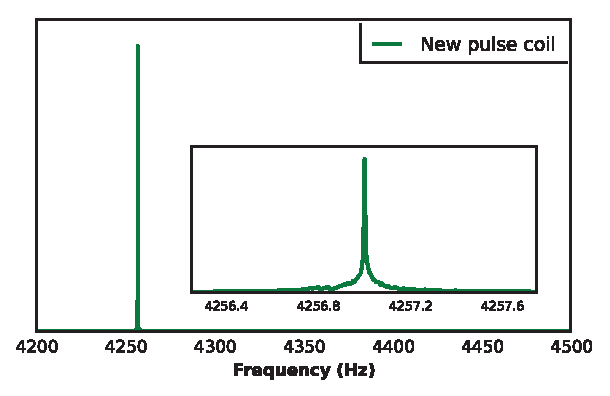
\includegraphics[width=\tw]{figures/coils/PCHomogeneityCompNX.eps} \\
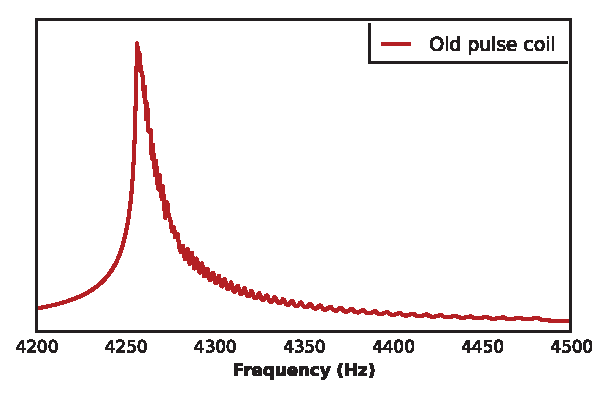
\includegraphics[width=\tw]{figures/coils/PCHomogeneityCompOX.eps} 
\end{tabular}
\caption{X Coil}
\label{fig:PCHomogeneityComparisonX}
\end{subfigure} 
\begin{subfigure}[h]{0.3\tw}
\begin{tabular}{c}
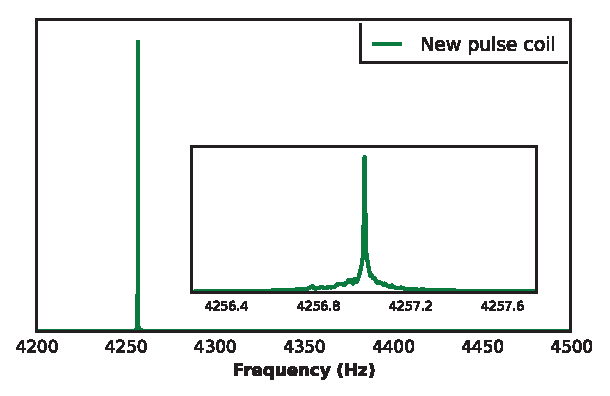
\includegraphics[width=\tw]{figures/coils/PCHomogeneityCompNY.eps}\\
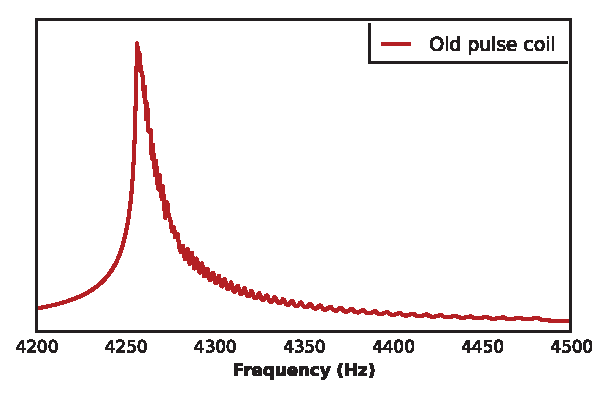
\includegraphics[width=\tw]{figures/coils/PCHomogeneityCompOY.eps}
\end{tabular}
\caption{Y Coil}
\label{fig:PCHomogeneityComparisonY}
\end{subfigure}
\begin{subfigure}[h]{0.3\tw}
\begin{tabular}{c}
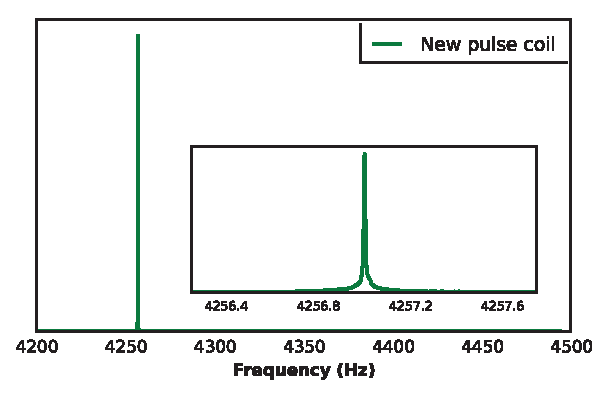
\includegraphics[width=\tw]{figures/coils/PCHomogeneityCompNZ.eps} \\
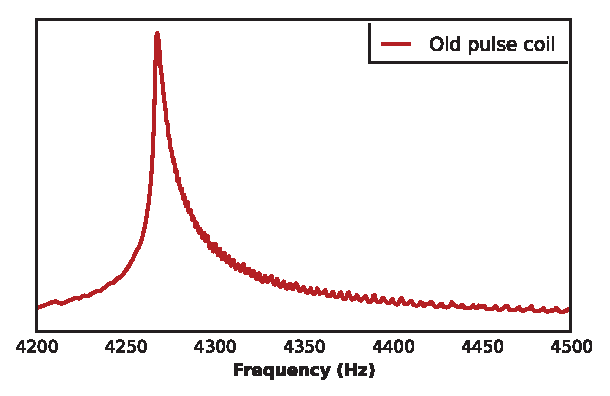
\includegraphics[width=\tw]{figures/coils/PCHomogeneityCompOZ.eps}
\end{tabular}
\caption{Z Coil}
\label{fig:PCHomogeneityComparisonZ}
\end{subfigure}\\
\caption{A comparison of the predicted pulse coil inhomogeneity. These spectra are generated by simulations of the proton precession frequency over the sample volume, weighted by $\sfrac{1}{r^3}$ where $r$ is the distance between a given point in the sample volume and the center of the sensitive magnetometer volume.}
\label{fig:PulseCoilHomogeneityComparisonFFT}
\end{figure}
The larger coils were designed in response to homogeneity concerns about the smaller coils. The smaller set of coils was made from a \unit[2]{"} diameter \unit[3]{"} height cylinder, with orthogonal \unit[0.5]{"} holes centered longitudinally (\unit[1]{"} from the top and bottom). Grooves \unit[$\sfrac{1}{16}$]{"} deep were used for all coil windings. Helmholtz pair geometry is constrained such that the coil separation $\Delta z = r$, where $r$ is the radius of each loop. Assuming that a single layer of \unit[30]{AWG} wire is used in a \unit[$\sfrac{1}{16}$]{"} groove, the separation between the centers of the Helmholtz grooves was set to \unit[0.9425]{"}.  The saddle coils were wound with \unit[120]{\degsym} angular extent along grooves wound at the top and bottom edges of the coil substrate. The radius depends somewhat on the way the coils are wound, but is $\approx$ \unit[0.9375]{"}, with heights of \unit[1.875]{"}, for an $\frac{h}{r}$ ratio of 2, far from the optimal value of 4 described in \emph{Ginsberg et al., 1970}\cite{Ginsberg1970}.

Another factor leading to significant inhomogeneity is that the original coil designs did not take into account the fact that the pulses are to be applied to the \textit{sample}, rather than the cell. In the most recent design of the magnetometer, the bottom of the sample tube is approximately \unit[0.1]{"} (\unit[2.5]{mm}) from the top of the cell; when filled with a volume of \unit[100]{$\mu$L}, the height of the fluid in the tube is $\approx$ \unit[0.31]{"} (\unit[8]{mm}) from the bottom of the tube. The homogeneity of a Helmholtz coil is greatest at the center, with the field dropping off by around \unit[150]{ppm} $\pm$ \unit[10]{\%} of the radius away from the center, and by \unit[2300]{ppm} at $\pm$\unit[20]{\%}. Since the radius of the original pulse coils was \unit[1]{"}, the sample being centered $\approx$ \unit[0.25]{"} above the coil center, and thus would be in the inhomogeneous fringe field. When the new, larger coils were designed, the pulse coils were thus centered \unit[0.25]{"} above the center of the optical access coils.  Combined with the increase in the coil radius and the optimization of the $\sfrac{h}{r}$ ratio for the saddle coils, the pulse homogeneity across the sample increased dramatically, as seen in the simulations plotted in \Cref{fig:PulseCoilHomogeneityComparisonFFT} (which are consistent with observations).

The blueprints for both sets of coils can be found in \Cref{blueprints}; the new pulse coils are Figures \ref{blueprints:NewPulseCoils01} and \ref{blueprints:NewPulseCoils02}, the smaller pulse coils are Figure \ref{blueprints:OldPulseCoils},

\subsection{Substrates and Materials}
\label{nmr.pulsecoil.substrates}
These coils are all wound on cylindrical substrates with grooves to accommodate magnet wire. The choice of material for the substrate is strongly constrained by the fact that these coils are located in the sensitive detection region. Magnetic materials cannot be used at all inside the shields, as they generally become magnetized, inducing large (relative to the sensitivity of the magnetometer) bias fields and gradients. Non-magnetic metals like copper and aluminum can be used if absolutely necessary, but the presence of large conductive bodies tends to induce large amounts of Johnson noise and limit the sensitivity of the device. Additionally, depending on the optimal cell operating temperature and thermal equilibrium characteristics of the system, the temperature in the sensitive region will often be very elevated, particularly near the cell itself - as such, all the system components must be designed to operate at high temperatures.

\begin{figure}[p]
\centering
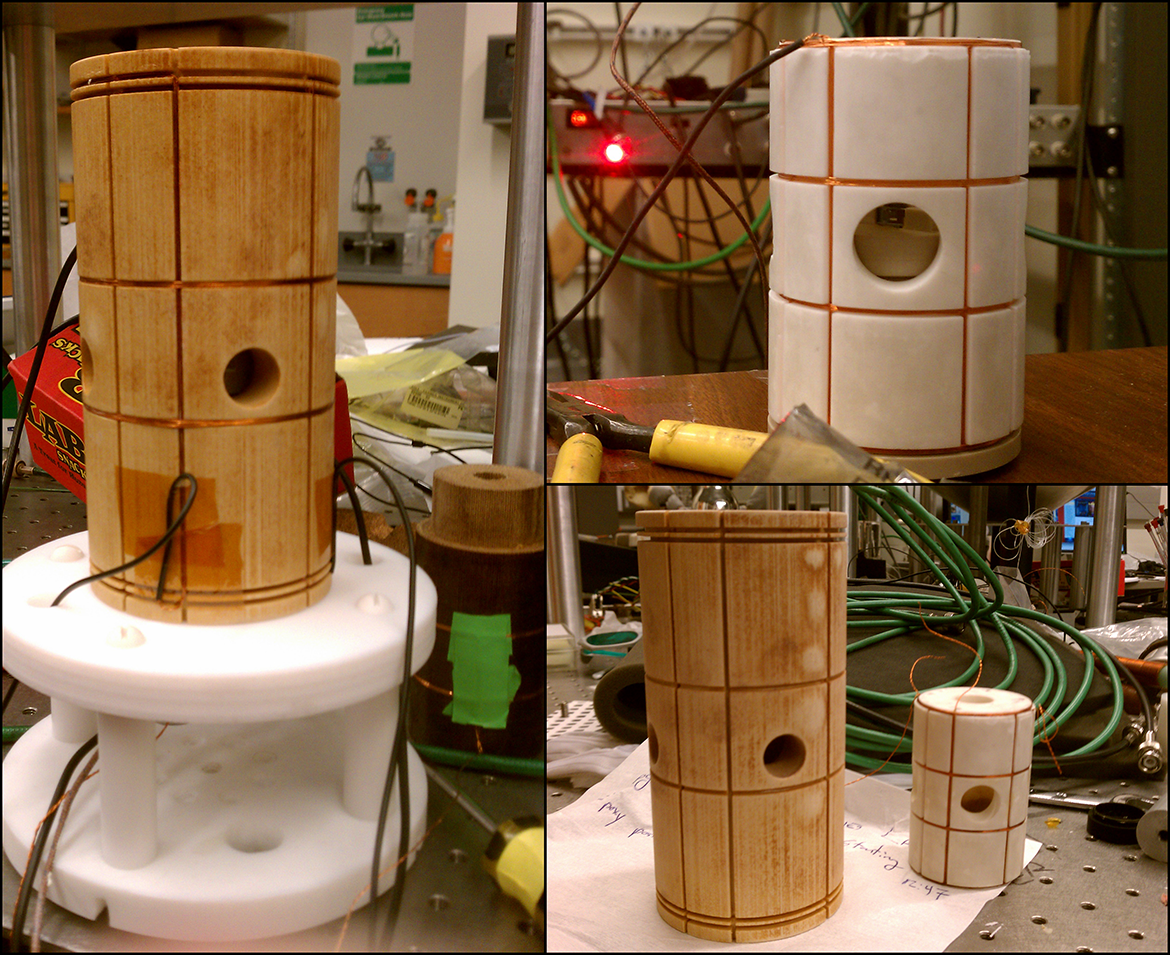
\includegraphics[width=\tw]{figures/magnetometer/PulseCoilsCollageSmaller.png}
\caption{Photographs of the new pulse coil assembly (left), old pulse coil assembly (top right) and a comparison between the new and old substrates (bottom right).}
\label{fig:PulseCoilPhotos}
\end{figure}

In our systems, most components are made of a combination of ceramics, high-temperature plastics and fiberglass, each of which has its own advantages. Ceramics are particularly attractive for their physical properties - they can be made as thermal insulators or conductors as needed, they are often quite rigid and have low thermal coefficients of expansion. However, there very few ceramics which can be easily machined, which is a significant constraint in custom applications such as this (though may not be so in bulk industrial production where they can be cast). Fiberglasses such as Garolite can be quite strong and rated to high temperatures. These have many favorable properties, but tend to be avoided when possible because although they are easier to machine than ceramics, doing so can represent a health hazard if the fibers enter the lungs. 

In most cases, the best material to use is a high-temperature plastic. In our magnetometers, we generally use either PTFE (Teflon, polytetrafluoroethylene) or PEEK (polyetheretherketone), though these are by no means the only high temperature plastics available. PTFE is extremely common, and so it is relatively inexpensive and frequently available in many forms, making it easy to find appropriate starting materials for a given part. PTFE is generally rated for use up to $\approx$ \unit[300]{\degsym C}, and is a good thermal insulator (with a thermal conductivity of \unitfrac[0.25-0.35]{W}{m$\cdot$K}), but it tend to have a very high coefficient of thermal expansion (\unit[135]{$\cdot\mathrm{10}^{-6}\mathrm{K}^{-1}$}), and is very slippery - both of which make it very difficult to machine with great precision. Acetal (Delrin) tends to have similar physical properties to PTFE, but with somewhat better friction, and so may be a good replacement if available. PEEK has similar thermal properties - \unitfrac[0.25]{W}{m$\cdot$K} thermal conductivity and a slightly better \unit[60]{$\cdot\mathrm{10}^{-6}\mathrm{K}^{-1}$} coefficient of thermal conductivity - but has much better friction, and can be much more easily machined. Additionally, PEEK is much less pliable than PTFE, giving much greater tolerances on objects with thin feature sizes, as well as making such objects more robust.

In the latest version of the pulse coil, the substrate was 3D printed using a 3D Systems Z-Printer 150, which uses ink jet technology to selectively bind successive layers in a powder bath, and when complete, the part is infused with a hardening epoxy. The physical properties of the object are primarily determined by the epoxy, and so can be varied depending on what is desired. Although there are a set of well-tested epoxies frequently used with Z-Printer models, any epoxy or resin can theoretically work. Generally a primary concern is the fluid viscosity, as this will determine the degree to which the epoxy can penetrate the material. Most commonly-used epoxies as hardeners are not rated for high-temperature use, and so a special high-temperature epoxy was used.\footnote{At the time, no high temperature epoxies were available from 3D Systems, and so I obtained from the local representative a sample of epoxy intended to be tested for high-temperature use. Other than some scorching during the higher-temperature baking process, the epoxy performed well, and there were no structural problems with the resulting parts.} These epoxies generally have a certain temperature hysteresis response, and so they are hardened by sequentially baking and cooling the part progressively until the desired temperature rating was achieved. In our tests of the epoxy some outgassing and scorching were observed during the baking procedure, but in nearly a year of constant use at $\approx$ \unit[90-150]{\degsym C}, no distortions have been observed.

The primary advantages of 3D printing of parts are time and cost, as the marginal cost of production of a given part is quite low, and printing is often quick - this is particularly advantageous in technology development applications, where prototype production may be a limiting step. However, currently the library of materials available for commercial 3D printing applications is very limited, which is a significant constraint on its potential use. 

\subsection{Pulse Generation Circuit}
\label{pulse.circuit}
% History of the various circuit designs.
\begin{figure}[h!]
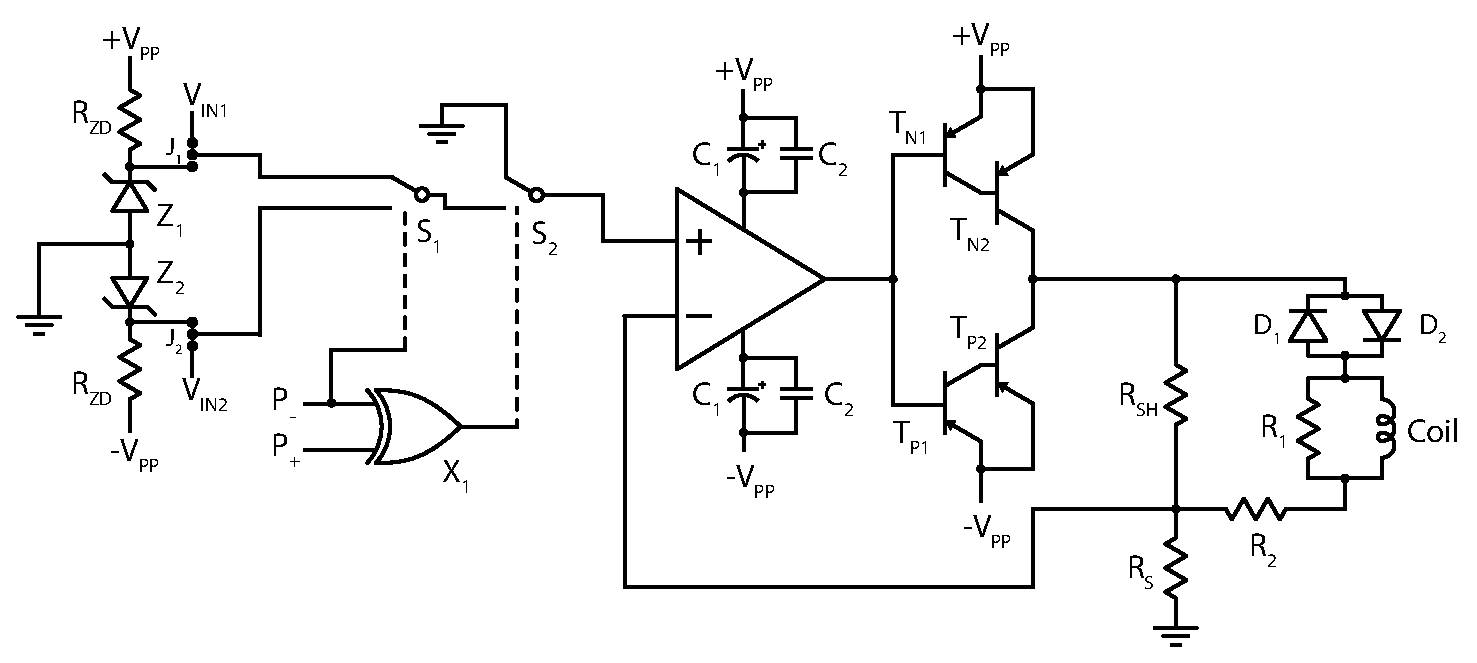
\includegraphics[width=0.95\tw]{figures/magnetometer/PulseCircuitFinal.eps}
\caption{The most recent version of the Pulse Coil Circuit}
\label{fig:PulseCoilCircuitFinal}
\end{figure}

Pulse control circuitry can be one of the most difficult aspects of magnetometer design as it has many significant challenges. Pulses generally need to be fast, precisely timed, strong, stable, extremely reproducible and not distorted - and produce very little noise. Depending on the purpose of the pulses, one may also be concerned with linear input response, AC performance and output symmetry.

When pulse length may present a problem for a given set of experiments, it is preferable to use extremely strong pulses. This is desirable for example in situations where large numbers of pulses are used, as longer pulses will take up a comparatively greater fraction of the experiment time and may impose limits on the experiment. An example of such problems is provided in section \ref{relaxation.t2.cpmg.pulse.time}, wherein pulsing-time fraction can effect measured relaxation properties. Strong pulses are also valuable for several J-spectroscopy applications wherein spins are addressed by their differential gyromagnetic ratio ($\gamma_I - \gamma_S$) rather than the gyromagnetic ratio of either spin - the closer the two values, the longer the pulse needs to be. One significant downside of using strong pulses is that timing errors produce larger pulse angle errors, as they make up a larger fraction of the pulse. High-powered pulsing applications also require much more care in their design, as the thermal properties of both the components and the coil become important as large currents are passed through them. In general, however, the main limit on our pulsing power has not been the circuit design, but rather the fact that strong pulses tend to magnetize the shields, changing the magnetic environment and interfering with our signal.

The circuit we use is a 4-channel bi-directional TTL-controlled pulse generator which was designed primarily for stability and versatility, as it is used in many experiments on multiple instruments, and often for multiple purposes within a single experiment. It can be used to deliver either DC or low-frequency RF pulses (the frequency cutoff is determined by the gain bandwidth of the op-amp), with maximal symmetry between positive and negative output. The circuit for each channel (which is shown in Figure \ref{fig:PulseCoilCircuitFinal}) is divided (roughly) into three stages: an input stage, an amplification stage and an output compensation stage.

\subsubsection{Input Stage}
\label{pulse.circuit.input}
\begin{wrapfigure}{L}{0.35\textwidth}
\vspace*{-0.5\lineheight}
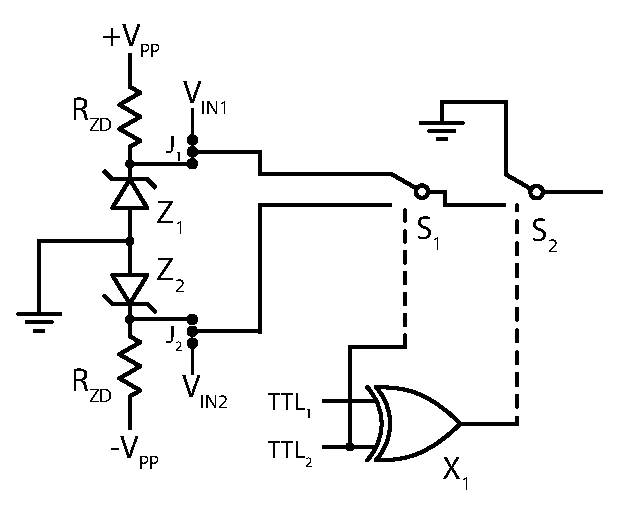
\includegraphics[width=0.35\textwidth]{figures/magnetometer/PulseCoilCircuitInputStage.eps}
\caption{Input stage of the pulse coil circuit}
\label{fig:pulse.circuit.inputstage}
\vspace*{-1.5\lineheight}
\end{wrapfigure}This circuit is a bi-directional TTL-controlled DC pulse generator with the option to configure each pulse ``direction'' using either a fixed DC level or an analog voltage input. In the physical realization of the circuit, the mode of a given channel is chosen by jumpers J$_1$ and J$_2$, as the decision to switch a channel (or half a channel) DC and voltage-controlled currents tends to be semi-permanent. These could also be replaced with physical switches without much issue.

The pulsing is controlled by a pair of TTL-controlled double-pole single throw break-before-make analog switches (MAX319). S$_1$ controls the input voltage channel and S$_2$ enables a pulse. The TTL-level voltage inputs (TTL$_1$ and TTL$_2$) feed into an exclusive-OR switch, which controls the analog switch (S$_2$). The S$_1$ switch is directly controlled by the channel corresponding to the ``normally closed'' input channel (in this case TTL$_2$ - this ensures that when it needs to be activated the S$_1$ switch will always switch \emph{before} the S$_2$ switch, as the XOR introduces a short delay into the logic propagation.

The fixed-voltage inputs are provided by a pair of reference Zener diodes, in our application these had a voltage drop of \unit[5]{V}. The current drawn from these inputs is small, and so the current-limiting resistors $\mathrm{R}_{\mathrm{ZD}}$ can be large. Depending on the application, it would likely be appropriate to add current-limiting resistors and/or protective optocouplers to the arbitrary voltage inputs.

\subsubsection{Amplification Stage}
\label{pulse.circuit.amplification}
\begin{wrapfigure}{r}{0.33\textwidth}
\vspace*{-0.7\lineheight}
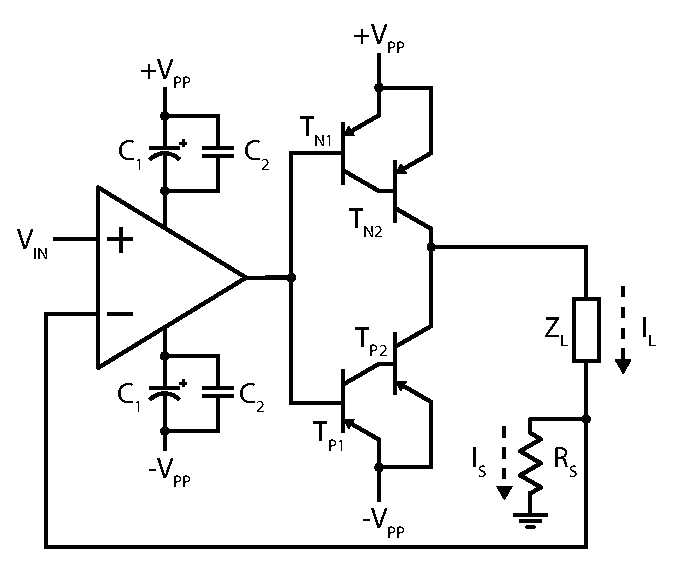
\includegraphics[width=0.33\textwidth]{figures/magnetometer/PulseCoilCircuitAmpStage.eps}
\caption{Equivalent circuit of the amplification stage of the pulse coil circuit.}
\label{fig:pulse.circuit.ampstage}
\vspace*{-0.5\lineheight}
\end{wrapfigure}The selected input channel is then fed into an operational amplifier configured as a voltage-controlled current source. To supply the often significant current required for strong, square pulses, a push-pull output circuit is wired within the feedback of the operational amplifier. In previous circuits, the current amplification took place outside the feedback stage, as the base turn-on junction of the transistors serves to filter out noise on the inputs of the operational amplifier. However, there are several distinct disadvantages as well --- one primary drawback is that when used outside the feedback loop, the actual current output during the pulses will depend on the specific conduction and amplification characteristics of the transistor - which can introduce short-term drift into the pulse calibrations as the transistors heat up, as well as long-term drift in the calibrations as the transistors age. 

When included in the feedback loop, the op-amp output compensates for the specific characteristics of the transistors, providing consistent output. An additional advantage to this configuration is that it allows an AC signal to be passed as a voltage input without much output distortion, as the op-amp output effectively eliminates the diode drops in the push-pull stage which normally severely distort AC output. Such AC signals would, however, be limited to fairly low frequencies, however, as the op-amp is required to slew very quickly when the output signal is in the transitory region between $\pm$2$\cdot$V$_\mathrm{D}$ (or $\pm$V$_\mathrm{D}$ when using Sziklai rather than Darlington pairs in the push-pull circuit).

\subsubsection{Output Stage}
\label{pulse.circuit.output}
\begin{wrapfigure}{l}{0.33\textwidth}
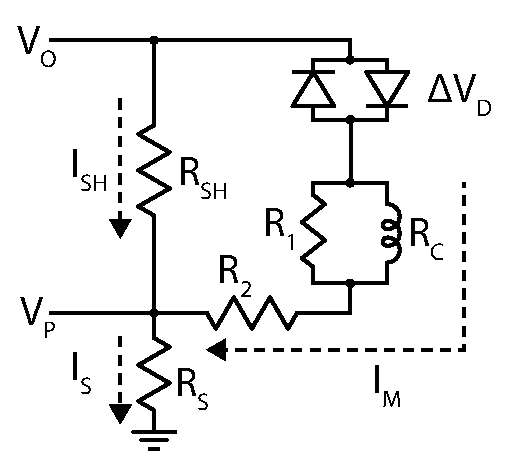
\includegraphics[width=0.33\textwidth]{figures/magnetometer/PulseCoilCircuitOutputStage.eps}
\caption{The output stage of the pulse coil circuit.}
\label{fig:pulse.circuit.outputstage}
\vspace{-0.1\lineheight}
\end{wrapfigure}

To eliminate noise from the logic and push pull stages of the circuit, anti-parallel diodes are placed in series with the coil, introducing a \unit[0.5]{V} voltage drop between the output of the push-pull stage and the input to the coil. A shunt resistor ($R_{SH}$) is in parallel with both the coil and the diodes, and for any current such that $I\cdot R_{SH} < \Delta V_{D}$, all current flows only through the shunt resistor and not through the coils. Above the diode drop voltage, the fraction of the current passing through the shunt resistor is given by

\begin{equation}
\label{eqn:pulse.coil.circuit.shunt.current.alt}
\frac{I_{SH}}{I_{SH} + I_{M}} = \frac{V_{P}R_{M} + \Delta V_{D}R_{S}}{V_{P}(R_{M} + R_{SH})},
\end{equation}

which quickly dies off with the pulse strength. Ideally $R_{SH}$ is set such that the the maximum values of the noise current generate voltages on the order of $\Delta V_D$, as this minimizes current passing through the shunt current and reduces distortion in AC cases and when applying low-intensity pulses.

\section{Field Shimming}
\label{mag.design.shimming}
\subsection{Shim Coils}
\label{mag.design.shim.coils}
In order to operate at zero field (or at an arbitrary but chosen field), it is necessary to shim out any remaining fields or field gradients resulting either from residual external magnetic fields or the slight magnetization of the shields. In this magnetometer, we use a tri-axial set of coils wound on a PTFE substrate to shim the field to the desired levels in each direction. No gradient shims are wound because no ill effects of residual gradients have been observed in these experiments.

\subsubsection{Design}
\label{mag.design.shim.coils.design}
%The design of the coils, simulations of their homogeneity, exploration of the mirroring effect.
\begin{figure}[ht!]
\centering
\begin{subfigure}[b]{0.3\textwidth}
\centering
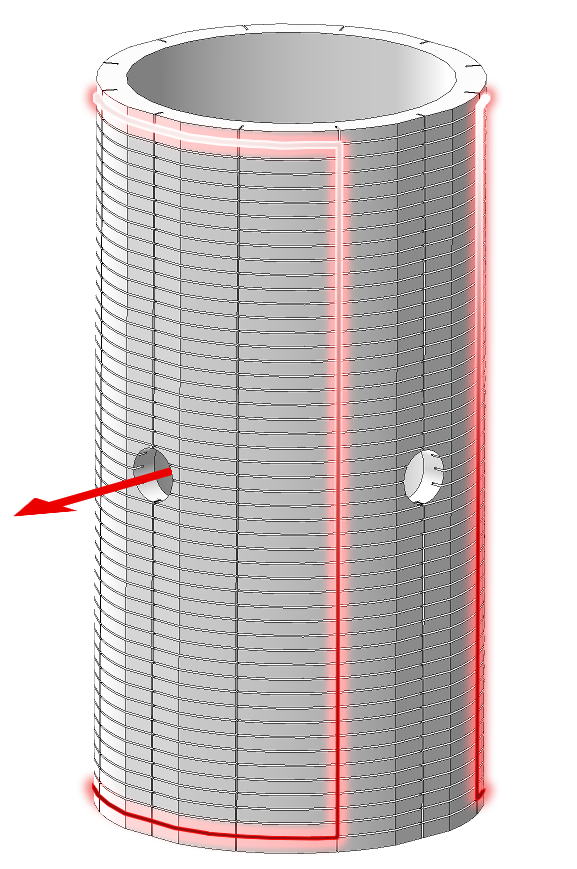
\includegraphics[width=\textwidth]{figures/magnetometer/FieldCoilX.png}
\caption{}
\label{fig:FieldCoilX}
\end{subfigure}
\begin{subfigure}[b]{0.3\textwidth}
\centering
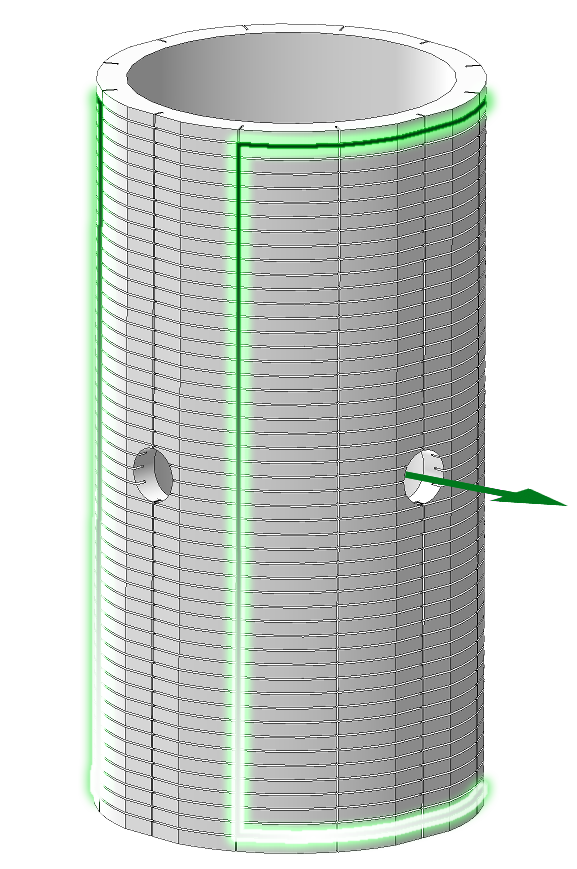
\includegraphics[width=\textwidth]{figures/magnetometer/FieldCoilY.png}
\caption{}
\label{fig:FieldCoilY}
\end{subfigure}
\begin{subfigure}[b]{0.3\textwidth}
\centering
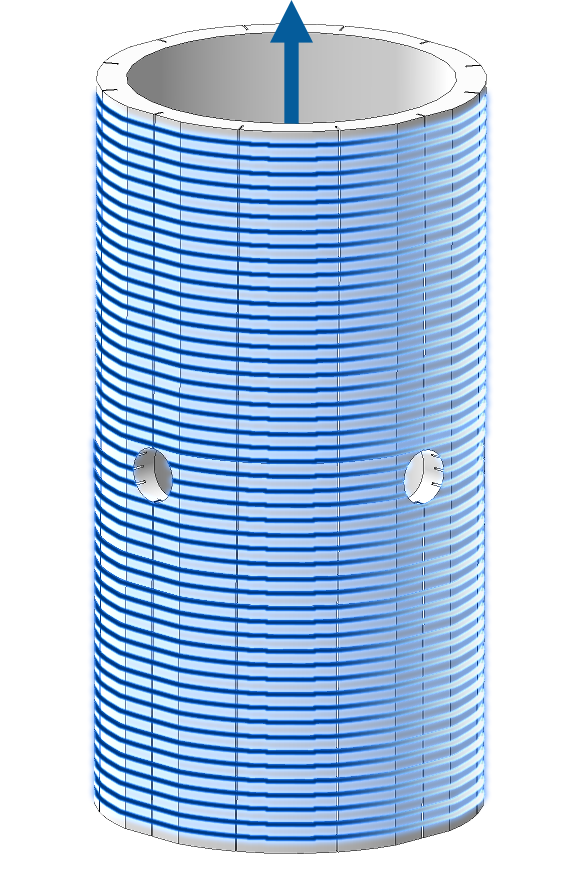
\includegraphics[width=\textwidth]{figures/magnetometer/FieldCoilZ.png}
\caption{}
\label{fig:FieldCoilZ}
\end{subfigure}
\caption{The coil windings are shown for the $x$ (\subref{fig:FieldCoilX}), $y$ (\subref{fig:FieldCoilY}) and $z$ (\subref{fig:FieldCoilZ}) coils.}
\label{fig:fieldcoils}
\end{figure}

The shim coils are wound from \unit[30]{AWG} copper magnet wire on a PTFE substrate which has a height of \unit[12]{"} (\unit[30.48]{cm}), an inner diameter of \unit[5.5]{"} (\unit[13.97]{cm}) and an outer diameter of \unit[6]{"} (\unit[15.24]{cm}). Radial grooves $\tfrac{1}{16}$" (\unit[1.5875]{mm}) wide and \unit[$\tfrac{1}{4}$]{"} (\unit[6.35]{mm}) deep are cut at \unit[$\tfrac{1}{4}$]{"} intervals, starting \unit[$\sfrac{1}{8}$]{"} (\unit[3.175]{mm}) from the bottom of the substrate, with 12 additional longitudinal grooves arrayed at \unit[30]{\degsym} intervals. This substrate is intended to fit snugly inside the innermost shield, allowing the coils to be as big as possible to maximize homogeneity at the point of the cell. Optical access is granted via 2 sets of orthogonal \unit[0.93]{"}-diameter holes at the center (vertically) of the structure, and in order to accommodate weld seams at the point of the optical access holes in the shields, the 4 sides hosting optical access ports are milled down to a flat surface. Because the optical access holes are larger than the spacing between radial grooves, it is necessary for several of the ``z'' coil windings to avoid the optical access holes. In this design, a \unit[1]{"} ring groove surrounds each optical access hole, allowing the magnet wire to wind around the holes.

Three coils are wound on this structure (Fig. \ref{fig:fieldcoils}): the transverse coils use a ``saddle'' configuration to generate fields along $x$ and $y$, while the the longitudinal coil uses a solenoid-like configuration to generate fields along $z$. Each lobe of the transverse coils consists of 2 windings with \unit[120]{\degsym} extent, with radius of \unit[2.25]{"} (\unit[13.97]{cm}) and a height of \unit[11.75]{"} (\unit[29.845]{cm}), a ratio of 5.22:1, which deviates from the optimal value of 4:1. As a result, the homogeneity of the field created across the cell is \unit[109]{ppm}, as compared to \unit[66]{ppm} for an optimal 4:1 coil. However, since there are radial grooves every \unit[0.25]{"}, it is possible to re-wind the coils with a \unit[9]{"} height to get an optimal 4:1 ratio without creating a new structure. In any case 

The spacing of the longitudinal coils is designed keeping in mind that these coils are sitting inside a shielded environment with flat end-caps. These flat end-caps act as magnetic ``mirrors'', and since the distance from the end-caps is $\frac{1}{2}$ the distance between windings, this geometry is equivalent to an infinitely long solenoid with \unit[0.25]{"} inter-wire spacing. This configuration provides a very homogeneous magnetic field, with a calculated homogeneity of \unit[1.8]{ppm} across the volume of the cell.\footnote{This is across the entire volume of the TwinLeaf cell, \unit[5]{mm}$\times$\unit[5]{mm}$\times$\unit[8]{mm}, not the intersection of the beams, which is a smaller region within the cell.}

\begin{center}
\begin{table}
\centering
\begin{tabular}[0.85\textwidth]{|E{0.1\tw}|E{0.25\tw}|E{0.25\tw}|E{0.25\tw}|}
\hline
 & Res. ($\Omega$) & Ind. ($\mu$H) & Response (G/A)\\ \hline
 \textbf{X} & 2.5 & 12.7 & 0.101\\ \hline
 \textbf{Y} & 2.4 & 12.7 & 0.101\\ \hline
 \textbf{Z} & 18.1 & 709.8 & 3.92\\  \hline
\end{tabular}
 \caption{Physical properties of the shim coils}
 \label{tab:FieldCoilProperties}
\end{table}
\end{center}

\subsubsection{Control Circuit}
\label{mag.design.shim.coils.circuit}
%The design of the circuit.
\begin{wrapfigure}{l}{0.4\textwidth}
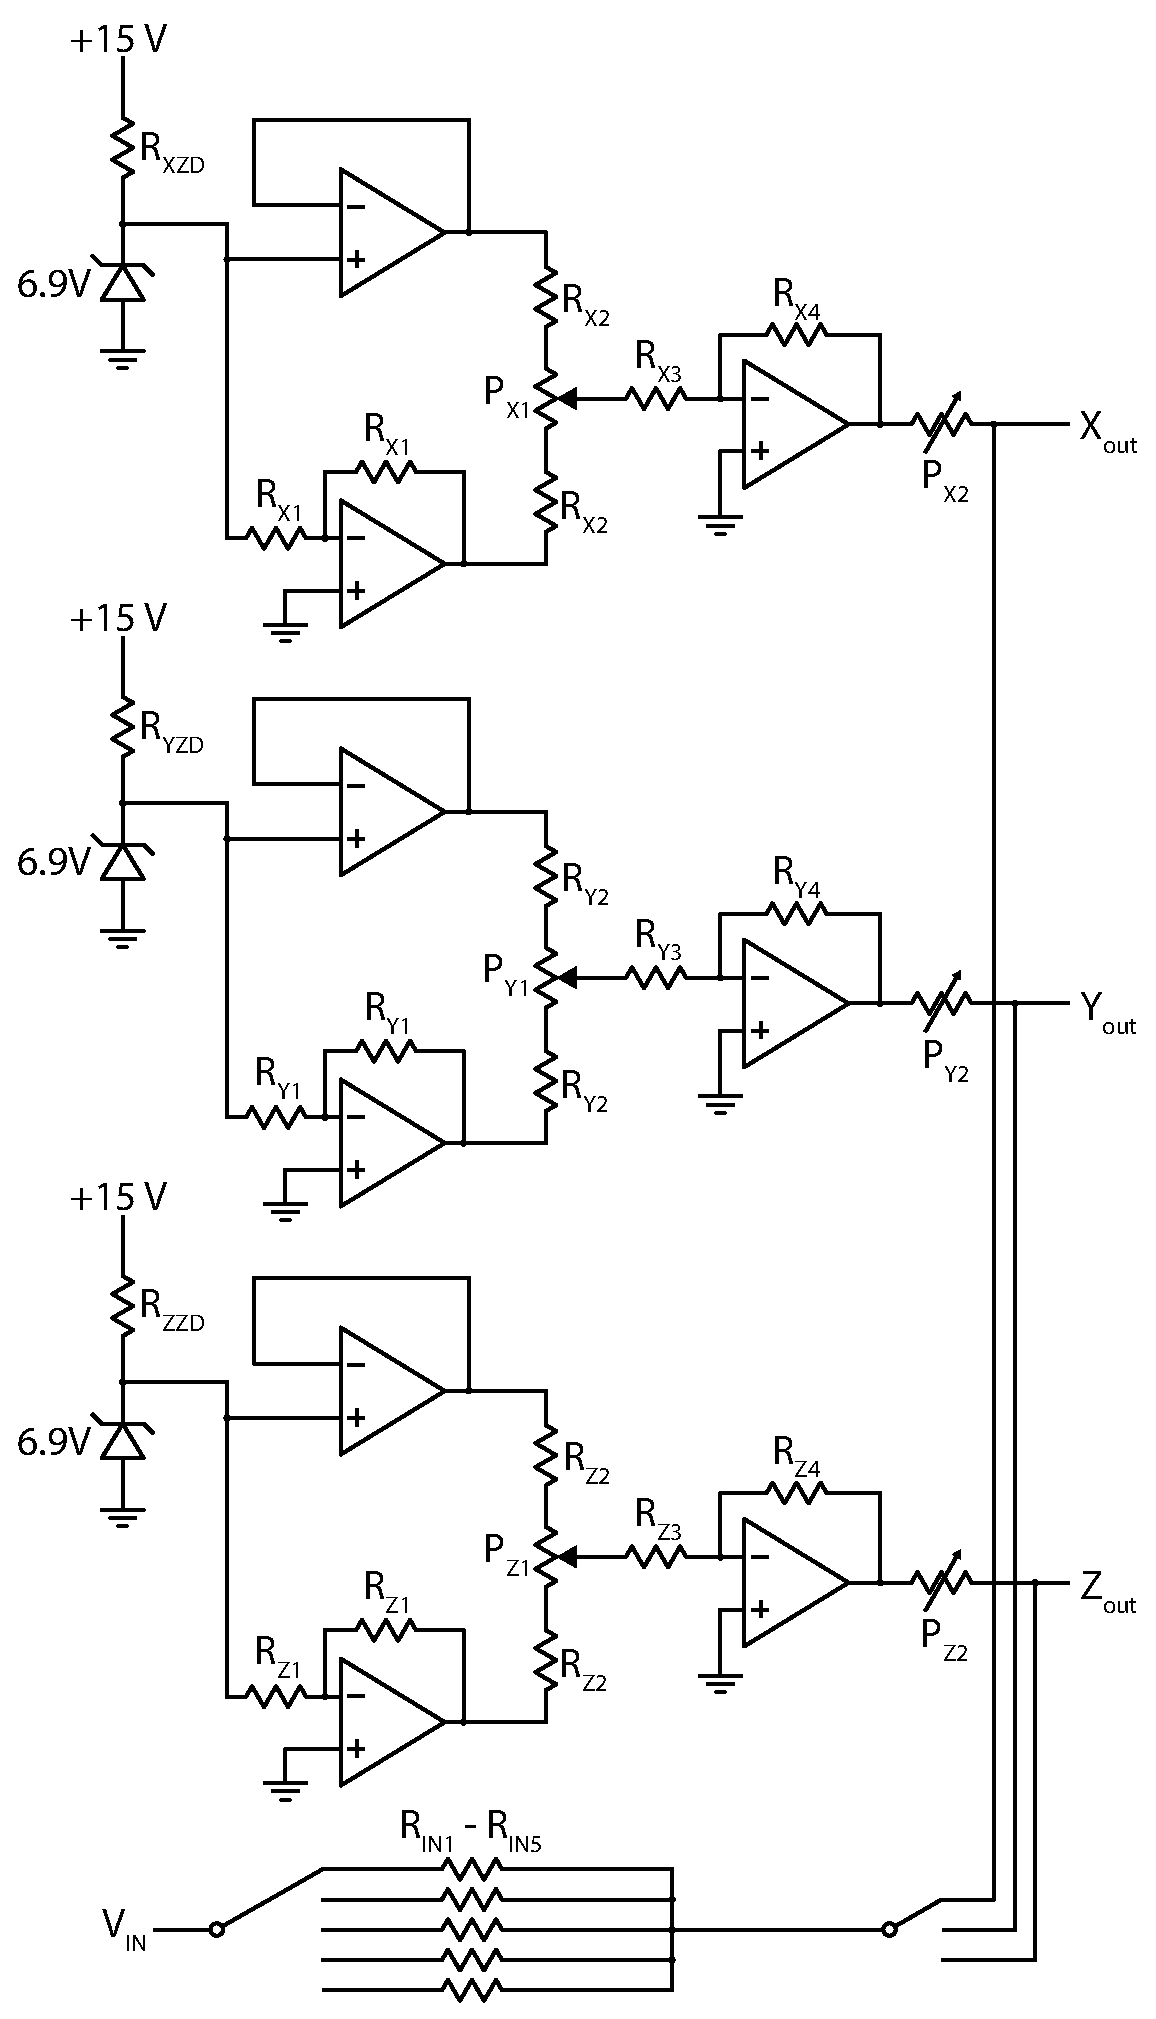
\includegraphics[width=0.4\textwidth]{figures/magnetometer/FieldCoilCircuit.eps}
\caption{The field coil circuit.}
\label{fig:FieldCoilCircuit}
\vspace{-0.5\lineheight}
\end{wrapfigure}

The shim coils are controlled with a homebuilt three-channel bi-directional op-amp current source (see \ref{fig:FieldCoilCircuit}), with the output voltage on each channel controlled by two independent potentiometers a coarse control (\emph{P$_{1i}$}) and a fine control (\emph{P$_{2i}$}). The output range of the circuit is limited by the choice of resistors, which is adjusted as-needed using a current-limiting potentiometer on the output (\emph{P$_{3i}$}). This is generally set such that the span of the output is limited to the voltage which produces a magnetic field spanning the sensitive region of the magnetometer, to give the finest control. 

\subsubsection{Noise Analysis}
\label{mag.design.shim.coils.circuit.noise}
There are two major sources of noise relating to the field coils, noise from the circuit and Johnson noise induced across the coils themselves. Depending on the specific configuration, either could be significant, and both can be reduced if they become limiting sources of noise. The Johnson noise current induced across a resisting wire is given by Eqn. \ref{eqn:JohnsonNoise}:

\begin{equation}
\label{eqn:JohnsonNoise}
I_{JN} = \sqrt{\frac{4k_BT\Delta f}{R}}
\end{equation}

Where $\Delta f$ is the bandwidth, $k_{B}$ is Boltzmann's constant, $T$ is temperature in Kelvin and $R$ is resistance. In the case of this design, this is a much more significant for the $z$ coil, which has a much greater magnetic response than the transverse ($x$ and $y$) coils. In the specific case detailed in \Cref{tab:FieldCoilProperties} at a temperature of 65\degsym C, the Johnson noise along the $z$ axis is \unitfrac[13]{fT}{$\sqrt{Hz}$}, and \unitfrac[0.87]{fT}{$\sqrt{Hz}$} along each transverse direction. This can be easily alleviated by choice of wire gauge, as resistance is inversely proportional to the cross-sectional area of the conductor and as such resistance decreases as the square of the wire radius. Thus switching from \unit[30]{AWG} (as was used here) to \unit[36]{AWG} would increase the resistance of the coil by a factor of $\approx$ 4, and reduce induced Johnson currents by a factor of 2 without affecting coil response or geometry - and as such would be advisable for situations where current is low enough that an increase in resistance would not cause damage to the coil. For significant increases in resistance, it might be necessary to adjust the limiting output resistor (P$_{Z2}$ in \Cref{fig:FieldCoilCircuit}) to compensate.

The second source of noise from the shim coils is noise from the circuit components - primarily the voltage reference and op-amps, as these are much more significant than noise from the resistors used in these circuits. The output current of the $z$ channel of the circuit detailed in \Cref{fig:FieldCoilCircuit} is given by the following equation:

\begin{equation}
I_{Z} = \frac{-R_{Z4}(P_{X2}+R_{Coil})}{R_{1}R_{2} - R_{Z3}(R_1-R_2)}\left[V_{ZD}(R_2 - R_1) + V_{O1}R_2 + V_{O2}\right] + V_{O3}\left(1-\frac{R_{Z4}}{R_{Z3}}\right) 
\end{equation}

Where $R_1 = R_{Z2} + P_{Z1}p$, $R_2 = R_{Z2} + P_{Z1}(1-p)$ and $0 \leq p \leq 1$ (representing the position of the potentiometer). The terms $V_{O1}$, $V_{O2}$ and $V_{O3}$ refer to the voltage offset input bias, and for the purposes of this error analysis are all set to $0 \pm \sigma_{OP}$. Using this, we can determine the overall noise $\sigma_{IZ}$ by propagating the errors from the op-amps and Zener diode references:

\begin{equation}
\sigma_{IZ} = \sqrt{\left(\frac{\delta I_{Z}}{\delta V_{ZD}}\right)^2\sigma_{ZD}^2 + \left(\frac{\delta I_{Z}}{\delta V_{O1}}\right)^2\sigma_{OP}^2 + \left(\frac{\delta I_{Z}}{\delta V_{O2}}\right)^2\sigma_{OP}^2 + \left(\frac{\delta I_{Z}}{\delta V_{O3}}\right)^2\sigma_{OP}^2}
\end{equation}

The Zener diode term comes out as:

\begin{equation}
\sigma_{ZD}^2\left(\frac{\delta I_z}{\delta V_{ZD}}\right)^2 = \frac{R_{Z4}^2(P_{X2} + R_{Coil})(R_2-R_1)}{[R_{1}R_{2} - R_{Z3}(R_1+R_2)]^2}
\end{equation}

The terms from the errors on the three op-amps are:

\begin{align}
\sigma_{amp} & = & \sigma_{op}\sqrt{\left(\frac{\dif I_z}{\dif V_{o1}}\right)^2 + \left(\frac{\dif I_z}{\dif V_{o2}}\right)^2 + \left(\frac{\dif I_z}{\dif V_{o3}}\right)^2} \\
& = & \sigma_{OP}\sqrt{(P_{X2} + R_{Coil})\left[\frac{R_{Z4}^2(R_1^2 + R_2^2)}{[R_1R_2 - R_{Z3}(R_1+R_2)]^2} + \left(1-\frac{R_{Z4}}{R_{Z3}}\right)^2\right]} \label{eqn:field.coil.OpAmpNoise}
\end{align}

One important thing to note is that due to the symmetry of the circuit, the noise from each component varies quadratically with $p$, but the error response from the op-amps is concave while the error response from the voltage reference is convex (see Fig. \ref{fig:ZFieldCoilNoise}). The op-amp noise is minimized at the extremes, because at those points there is only one source of noise, while at $p = 0.5$ the noise is maximized because there are equal contributions from two independent noise sources. Because the voltage reference provides identical noise to each side of the potentiometer, it is minimized at $p = 0.5$, where it is perfectly canceled.

Depending on the noise characteristics of available components, this analysis can argue for different configurations. The follower circuit branch of the current source is in place for added symmetry and to provide high output impedance for the next output stage. If these op-amps are the limiting noise source, however, modest gains may be achieved by removing the follower circuit, provided that sufficient current is supplied to the voltage reference (i.e. $R_{ZD}$ is sufficiently high).

\begin{figure}[ht!]
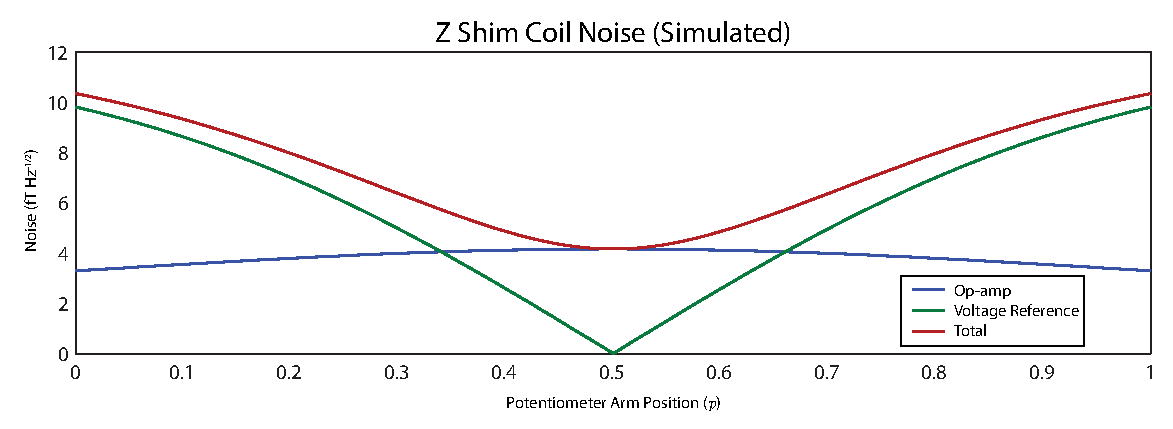
\includegraphics[width=0.95\tw]{figures/magnetometer/ShimCoilNoise.eps}
\caption{The expected circuit noise of the $z$ shim coil based on the current configuration with $\sigma_{ZD}$ = \unitfrac[100]{nV}{\rHz}, $\sigma_{OP}$ = \unitfrac[15]{nV}{\rHz}.}
\label{fig:ZFieldCoilNoise}
\end{figure}

\subsection{Field zeroing}
\label{mag.design.shim.coils.zeroing}
% Discussion of why SERF magnetometers should be operated at zero field, and why it is difficult.
\subsubsection{Applied Oscillation Method}
\label{mag.design.shim.coils.zeroing.oscillation}
%Description of the applied oscillation method of zeroing the fields.
Thanks to the vector nature of the SERF magnetometer, there is a simple way to make a preliminary zeroing of the transverse ($x$ and $y$ - see: \hyperref[terminology.coordinates]{Choice of Coordinates}) fields using the magnetometer signal alone. The magnetometer signal is given by the spin projection along the probe beam direction\cite{Seltzer2004}, which is
\begin{equation}
\label{oscillation.serf.spinprojection}
S_x = S_0\frac{\beta_z + \beta_x\beta_y}{1 + \left(\beta_x^2 + \beta_y^2 + \beta_z^2\right)},
\end{equation}

where 
\begin{equation}
\label{oscillation.serf.definebeta}
\boldsymbol{\beta} = \left(\frac{\gamma^e}{R_{OP} + R_{rel}}\right)\mathbf{B}.
\end{equation}

As such, if an oscillating magnetic field is applied along the $x$ direction, to first order the amplitude of the magnetometer response will be modulated by the residual field in the $y$ direction, and if an oscillating magnetic field is applied along the $y$ direction, to first order the amplitude of the magnetometer response will be modulated by the residual field in the $x$ direction. These fields can then be zeroed by minimizing the amplitude of the observed oscillation, while the field in the $z$ direction can be zeroed using the DC level.

Note that this method should be applied iteratively, cycling through the $x$, $y$ and $z$ zeroing procedures until no further oscillations are observed. This method works best when the magnetometer is operating at closest to zero in all three directions, and as such with each iteration the accuracy of the method is increased.

\subsubsection{Sample NMR Precession Method}
\label{mag.design.shim.coils.zeroing.sample.nmr}
% Description of the sample signal decay method
Given accurately determined pulse times, one way to zero the fields transverse to the polarization direction is by observing the low-frequency NMR signal of a long-T$_2$ sample in the presence of a train of $\pi$ pulses spaced in increments of $\tau$. For $\tau \ll \gamma B_x$ a $\pi_x$ train acts as a spin lock along the $x$ direction, and spin precession is entirely attributable to a residual field along $B_y$. The $\vec{y}$ shim can then be adjusted until no precession is observed. 

This approach is potentially most strongly limited by the error on the $\pi$ pulses, as error in the $\vec{x}$ pulse will translate into error in the $B_{x}$ shim. For

\begin{equation}
\tilde{B_{x}} = -\frac{\epsilon_{x}}{\tau\gamma}
\end{equation}

Where $\tilde{B_{x}}$ is the offset bias field along x which accounts for a pulse error of angle $\epsilon_{x}$ along $\vec{x}$. Another potentially limiting factor in the accuracy of the calibration is the decay from the T$_1$ of the sample, as no NMR precession can be observed when $\omega \ll T_{1}$. For $\omega \ll \sfrac{1}{T_{1}}$, signal decay occurs faster than NMR precession, and differences in precession frequency cannot be easily observed. Generally, it is possible for pulse errors to be reduced such that the limiting factor on NMR precession observations is the low field $T_2$ of the sample.

That said, this is likely the most sensitive measurement of the absolute field at the sample, as it is not subject to light shifts or birefringence, and is an effect based purely on the local magnetic field. Using the proper pulse calibration sequences\footnote{See \Cref{nmr.pulsecal.multiplepulse} for more details on pulse calibration.}, the pulse error can be reduced to the digitization error on pulse lengths - and the effective pulse error can be reduced even further by application of error-correcting pulse sequences, when pulse length calibration is extremely important. Even greater calibration sensitivity can be achieved by using long-$T_1$ materials - the simplest thing to do is often to detect water at an elevated temperature, as its low field $T_{1}$ and $T_{2}$ are a strong function of temperature the samples, and so by either actively heating or reducing cooling mechanisms, the $T_1$ can be increased as needed.

Even the need for for accurate pulses can essentially be obviated at zero-field by using J-coupling spectra as the field probe; the theory of zero-field J-coupling spectroscopy is described in more detail in \Cref{nmr.signal.jcoupling}. Because there is no preferred axis for J-coupling spectra, the signal relies on the relative orientations of heteronuclei; as a result, spins undergoing incomplete excitation should simply not contribute to the J-coupling signals. When sufficiently small, deviations from zero field show up in J-spectra as perturbations, with the peaks split by the presence of the field.\cite{Ledbetter2011} The spectrum of \textsuperscript{13}C-labeled formic acid, for example, has a single peak at \unit[222]{Hz}, which is split into a doublet with peaks separated by $\delta\omega$ = $(\gamma_{H} + \gamma_{C})\mathbf{B_{0}}$ = \unitfrac[5328.1]{Hz}{G}$\cdot B_{0}$. Since the dependence on the field is linear for sufficiently small fields, the precise location of the required shim strength can be determined by making plots of the splitting frequency as a function of the field applied in each direction.

%\subsection{J-splitting Method}
%\label{mag.design.shim.coils.zeroing.jcoupling}
%
%\section{Bandwidth Measurement}
%\label{mag.design.bandwidth}
%
%\subsection{Frequency Sweep Method}
%\label{mag.design.bandwidth.frequency.sweep}
%The simplest method of measuring the magnetometer bandwidth is to apply a sinusoidal magnetic field and observe the amplitude and phase response of the magnetometer signal. The phase and amplitude are not necessarily related, and so it is worth recording both quantities for later use in phase-correcting NMR signals.\needexpand{Explain how to get a bandwidth number from the sweep numbers.}\needexpand{Mention possible pitfalls - photodiode bandwidth, low-pass filters, etc.}
%
%\subsection{Lorentzian Method}
%\label{mag.design.bandwidth.lorentzian}

\section{Cell Heating}
\label{mag.design.heating}
\begin{wraptable}{l}{0.5\tw}
\begin{tabularx}{0.5\tw}{|*{4}{Y|}}
\hline
 & A$_{\mathrm{mTorr}}$ & B$_{\mathrm{K}}$ & C$\mathrm{_{K}}$\\
 \hline
K$_{liq}$ & 14.114 & -4693 & -1.2403  \\
 \hline
Rb$_{liq}$ & 14.197 & -4275 & -1.3102 \\
\hline
Cs$_{liq}$ & 14.113 & -4062 & -1.3359 \\
\hline
\end{tabularx}
\caption{The coefficients which determine the alkali vapor pressure, based on Alcock et al.'s data.\cite{Alcock1984} Applying these coefficients to Eqn. \ref{eqn:VirialExpansionAlkali} for $T$ given in K returns $\mathrm{ln}\left(\tfrac{p}{mTorr}\right)$.}
\label{tbl:AlkaliCoefficients}
\end{wraptable}
Alkali vapor-cell magnetometers generally operate at an elevated temperature, as the temperature determines the vapor pressure of gaseous metal atoms through which the beams will pass. This is particularly important for spin-exchange-relaxation-free magnetometers, which operate in cells with a high density of buffer gas used to suppress spin-exchange relaxation\cite{Allred2002,savukov-optical-magnetometry-2013}. Experiments carried out on this magnetometer were performed with cells operating at temperatures ranging from \unit[155-195]{\degsym C}.

There are several ways that changing temperatures can affect signal and signal strength. Likely the most significant effect is the change in alkali vapor density, which depends strongly on the temperature. The alkali vapor density is given by:\cite{Alcock1984,Ewing1969}

\begin{equation}
\mathrm{log}\left(p\right) = A + \frac{B}{T} + C\cdot\mathrm{log}\left(T\right)
\label{eqn:VirialExpansionAlkali}
\end{equation}

Where $A$, $B$, and $C$ are the 1$^{\mathrm{st}}$-3$^{\mathrm{rd}}$ Virial coefficients. From literature values of these coefficients, it can be seen that the partial pressure (which is fairly directly related to the optical density of the cell) is a non-linear exponential function of the temperature. 

\begin{figure}
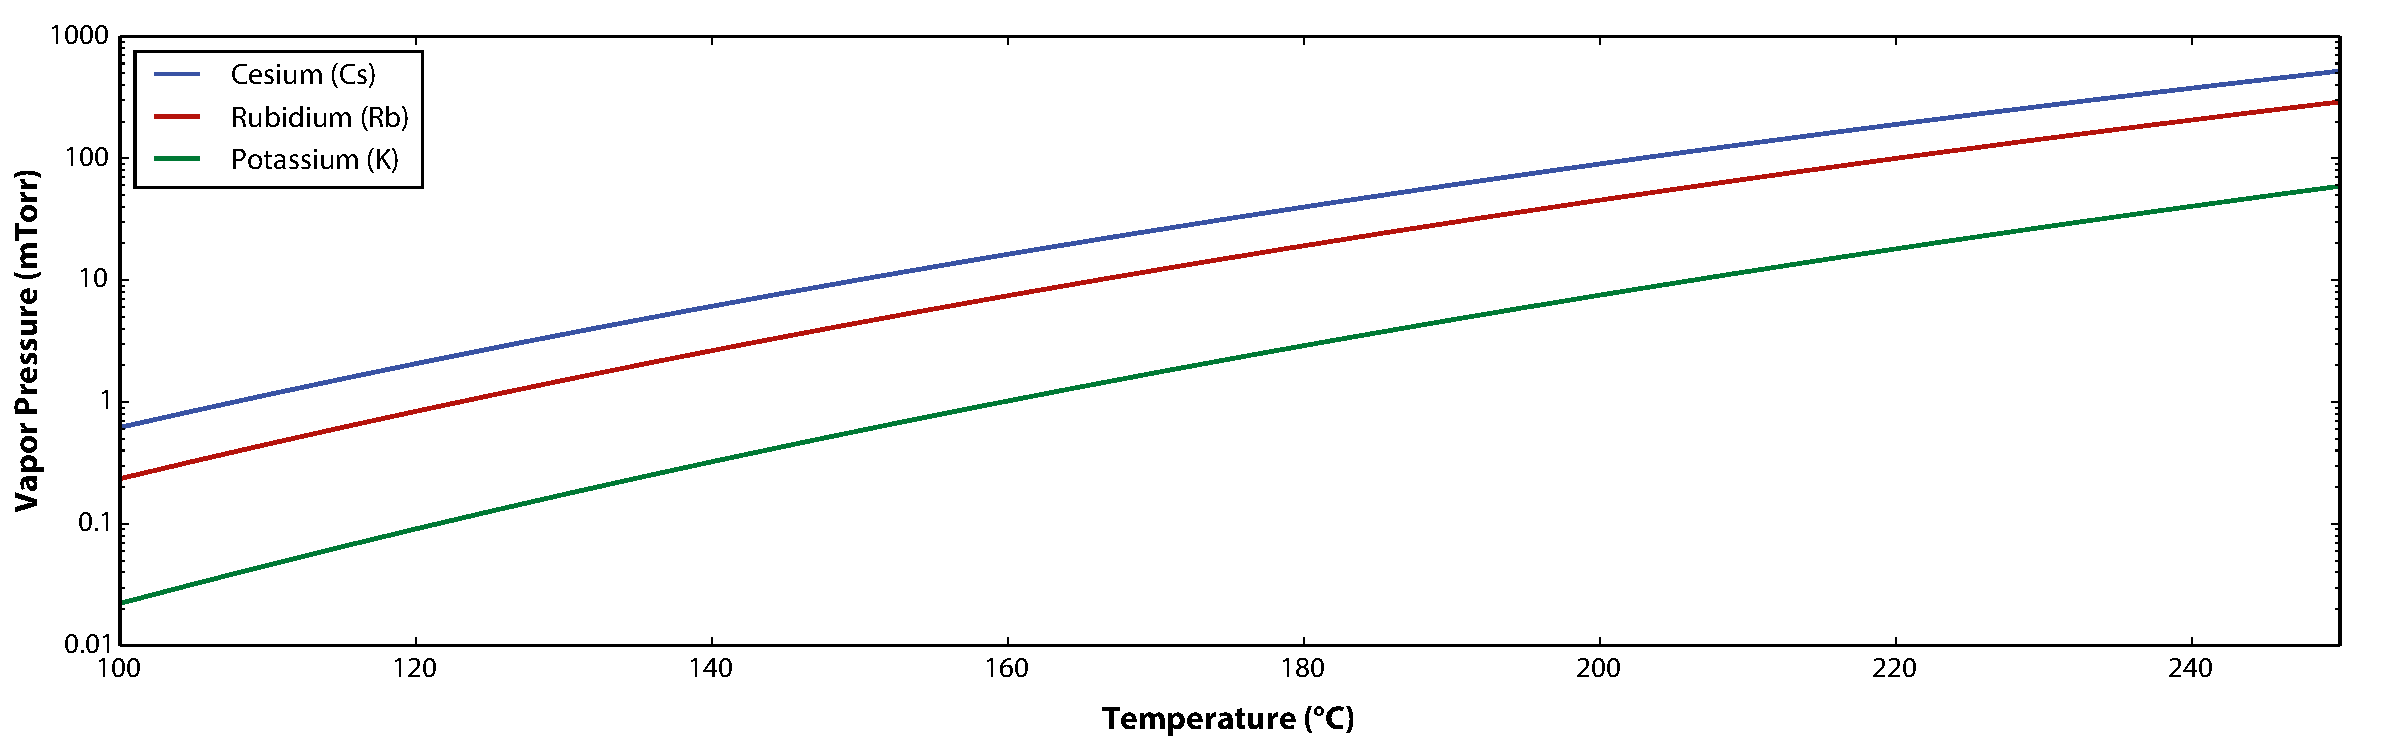
\includegraphics[width=0.95\tw]{figures/magnetometer/AlkaliVaporPressures.pdf}
\caption{The vapor pressure curves for the three alkali metals most commonly used in magnetometry. For low-temperature operations, Cesium is a natural choice, as the required vapor pressure can be created at much lower temperature.}
\label{fig:AlkaliVaporPressures}
\end{figure}

Creating such high temperatures introduces a number of challenges to the instrument design. Generally it is not desirable for samples or many common materials to be held at such high temperatures, but the fact that sample signal is inversely proportional to the cube of the distance from the cell precludes the use of significant insulation. Thus a situation wherein large temperature gradients are present is necessitated by the geometry of the instrument, and this can cause significant convection currents and induce birefringence in the cell's glass windows.\cite{Carusotto1984}

In addition to the problems caused by the elevated temperature, there are also challenges in producing the heating without introducing significant noise. There are two common approaches to this problem: resistive (coil) heating and laser heating. Resistive heating has two major significant problems - the current used to produce the heat will also produce a stray magnetic field, and the presence of enough metal to heat the cell will also likely introduce significant Johnson noise. Laser heating is highly preferable from a noise perspective, but can be very impractical for large cells and open geometries which require significant amount of power to heat. The heater designs used herein have required \unit[10--20]{W} of power, and it is difficult to find a material capable of efficiently transforming that amount of laser power into heat without ablating or otherwise becoming damaged. For smaller, microfabricated magnetometers, the power requirements can be on the order of \unit[100-200]{mW},\cite{Mhaskar2012,Schwindt2007} and in those applications, laser heating is practical and advantageous.

\subsection{Heater Design}
\label{mag.design.physical}
\begin{wrapfigure}{L}{0.3\tw}
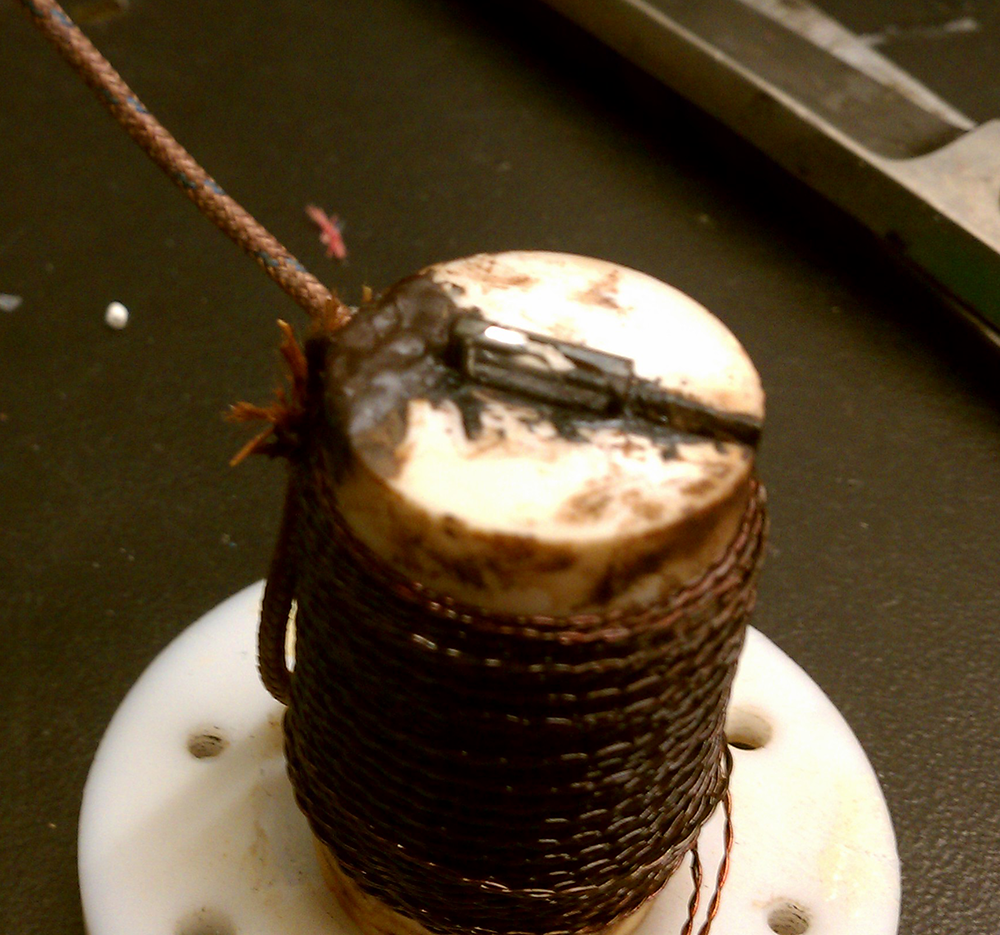
\includegraphics[width=0.3\tw]{figures/magnetometer/HeaterCoilVersion1-BrokenCellSmaller.png}
\caption{The original heater coil, with one of many shattered cells glued in place.}
\label{fig:OriginalHeaterCoilPhoto}
\end{wrapfigure}
The earliest design for the heater was a simple Macor rod with high-temperature-enamel-coated \unit[32]{AWG} twisted pair wire wound around it and a cell and thermocouple glued into a groove glued to the top, shown in Fig. \ref{fig:OriginalHeaterCoilPhoto}. The circuit was driven by the pulsed DC heater described in Sec. \ref{mag.design.pulsed.DC}. Among other reasons, this was found to offer inadequate protection to the magnetometer cell, resulting in the shattering of at least one cell during sample shuttling.

In order to minimize the possibility of heater shattering, a cap was added to the heater with offset stands upon which the probe head could sit, leaving $\approx$ \unit[100--200]{$\mu m$} space between the top of the cell and the bottom of the probe head, in an attempt to mechanically isolate the two. The cap was made of PEEK both for ease of machining and to thermally isolate the sample region from the heated cell. To cut down on thermal gradients, power consumption and thermally-driven air convection on the optical beam path, the rest of the heater was redesigned with thermal insulation in mind, given the significant size constraint that the entire heater apparatus needed to fit inside the small pulsing coil structure described in Sec. \ref{nmr.pulsecoil.designs} and shown in the top right panel of Fig. \ref{fig:PulseCoilPhotos}. 

\begin{figure}[ht!]
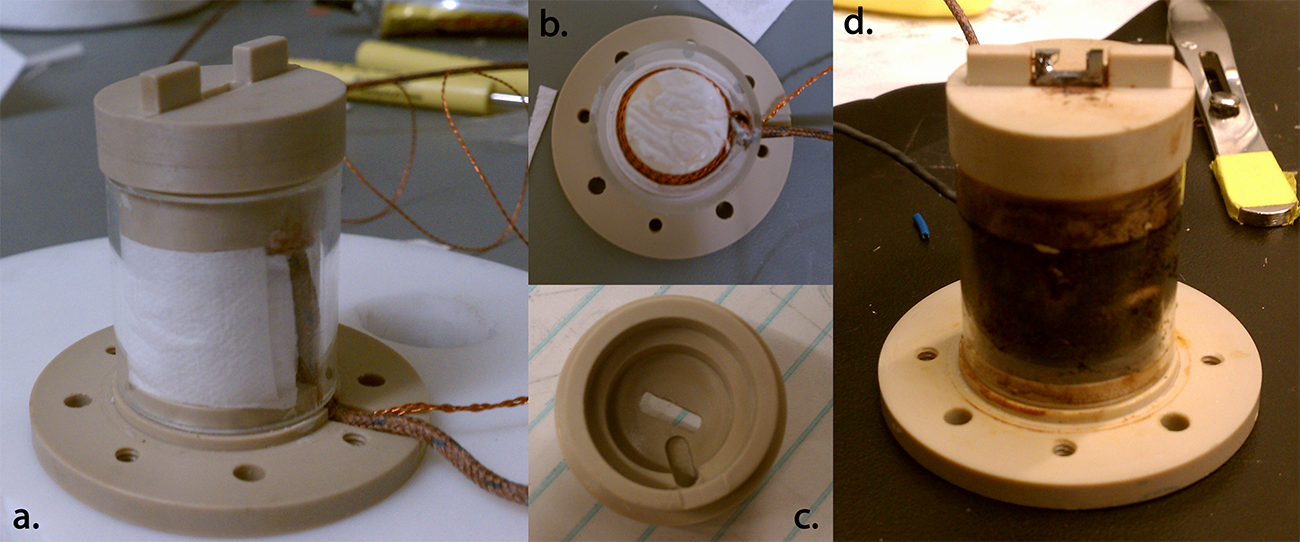
\includegraphics[width=\tw]{figures/magnetometer/HeaterSmallCellSmaller.png}
\caption{The second revision of the heater coil. a.) The assembled apparatus, with no cell in place b.) An overhead view of the wound coils, before the cap is added, but after high-temperature epoxy was applied to the heater coils c.) A view of the underside of the cap - a small notch is milled to accommodate the thermocouple d.) A view of a heater after use, with yet another shattered cell in place; the the extreme temperatures caused significant scorching of the insulating materials.}
\label{fig:RevisedHeaterCoilSmallCell}
\end{figure}

The first design change made was that the slightly thermally insulating Macor core (with a thermal conductivity \unitfrac[1.46]{W}{m$\cdot$K} and a specific heat of \unitfrac[0.8]{kJ}{kg$\cdot$K}) with a rod of thermally conductive aluminum nitride (which has a has a thermal conductivity of $\approx$\unitfrac[180--200]{W}{m$\cdot$K} and a specific heat of \unitfrac[0.75]{kJ}{kg$\cdot$K}). Because aluminum nitride is extremely hard and cannot be readily machined, it was not possible to mill a groove into the heater core that would accommodate a cell, and so the cell was primarily held in place by the cap itself. Rather than exposing the rod to air, in the first version of this design, the coil was wrapped in high-temperature fiberglass insulation, then a single layer of glass. The Teflon base was also replaced with a slightly thicker PEEK base. 

\begin{figure}[ht!]
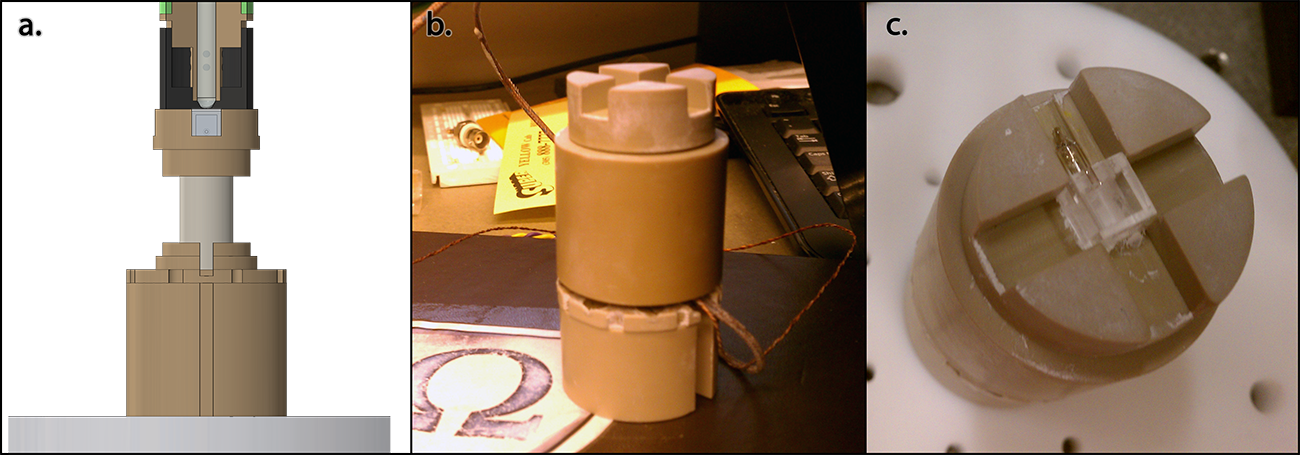
\includegraphics[width=\tw]{figures/magnetometer/HeaterLargeCellSmaller.png}
\caption{The version of the heater coil optimized for the larger ``cuvette''-style cells. a.) A render of the heater \textit{in-situ}, without coils or insulation. b.) A photograph of the wound and assembled heater c.) The cell in place on the heater; a small groove was added to one side of the heater cap to accomodate the cell's ``stem''.}
\label{fig:RevisedHeaterCoilLargeCell}
\end{figure}

When the microfabricated cell ($\approx$ \unit[7]{mm}$\times$\unit[4]{mm}$\times$\unit[2]{mm}) was replaced with a TwinLeaf ``cuvette''-style cell (\unit[7]{mm}$\times$\unit[7]{mm}$\times$\unit[12]{mm}), the heater needed to be redesigned again to accommodate the larger cell; the result is shown in \ref{fig:RevisedHeaterCoilLargeCell}. At this point, the smaller pulse coils were also replaced with a set of larger, more-homogeneous coils, relaxing the size constraint somewhat, allowing for more insulation around the heater. Because the microfabricated cell had only one optically-transparent surface, the original cap used small ``stands'' protruding from a mostly-flat cap to allow a wider array of input beam angles. The TwinLeaf cell was optically-transparent along all axes, and so the pump and probe beams passed through the cell normal to the glass surface, rather than at a \unit[45]{\degsym} angle; as such, only enough material was removed from the cap to allow the orthogonal beams to pass through, to maximize the volume of insulating material between the heater and the environment and sample. Additionally, a PEEK base was added below the heater, to accommodate for the increased height of the pulse coils. To improve the insulation, the fiberglass-and-glass casing was replaced with a thicker, PEEK case. This version was less fragile (the glass tubes would often break, either from differential thermal expansion or from mishandling) and added thicker thermal insulation. Additionally, since it is opaque, it helped to minimize the escape of heat in the form of infrared radiation. 

When the final version of the heater coil was first wound, the coil covered nearly the full length of the coil with 4 layers of wiring,\footnote{Only 2 layers of twisted pair wiring could fit between the coil and the inner diameter of the cap, so 4 layers were wound up the coil up to the point of the cap, then only two layers under the cap.} but this led to considerable noise on the magnetometer signal while heating, and so the coil was re-wound to cover only the bottom half of the core. This change did not seem to affect the apparatus's effectiveness. In earlier versions, the wires were initially held in place by superglue during winding,\footnote{The superglue would burn off at high temperatures, but by that point, the coils were tightly wound and/or held in place by a layer of fiberglass insulation, preventing it from spontaneously unwinding.} but in the final windings, this was replaced with high-temperature silicone heat sink compound, to increase the thermal conductivity between the layers and hopefully increase the effectiveness of the outer layers.

\subsection{Pulsed DC Heating}
\label{mag.design.pulsed.DC}
The initial design of heater circuit used a TTL-controlled pulsed DC heater. Leaving aside Johnson noise (which was not likely to be the limiting source of noise in these experiments), this would allow the magnetometer to operate without any potential stray fields from the heater. Since nearly all experiments done to date have had significant dead times for prepolarization and sample transfer, the heating pulses would not necessarily induce abnormally long experiment times.

The major downside, which ultimately made this approach impractical for these experiments, is that the cell cools over the course of the experiment, which serves to modulate many factors in the magnetometer's operation. This is particularly problematic for making measurements which require extremely high resolution where any single acquisition can go on for over a minute. This is somewhat problematic even in the case of short acquisitions, as temperature equilibration generally follows an exponential decay, and so much of the heat that will eventually be lost will be lost immediately after the heating is switched off.

Another issue with pulsed DC heating is that the mean steady-state temperature will depend on the duty cycle of the pulses - although generally all our heater circuits are configured as thermostats, equilibration after a change of duty cycle is not immediate, and this may introduce additional error into the measurements. With a sufficiently large heat reservoir and a long inter-pulse spacing, this is not an issue, but when sufficient time is not given for the temperature to stabilize after an experiment has finished, there will be some inevitable drift as the system finds a new equilibrium. Another strategy for dealing with this, however, is to maintain a constant duty cycle even when not conducting experiments, which allows the system to remain in equilibrium even when experiments start. This benefit, however, is tempered by the fact that this does not allow flexibility in the scheduling of experiments as the experiment timing is dictated by the heater's ``off'' period, rather than the heater's ``off'' period being dictated by the timing of the experiment.

\subsubsection{Pulsed DC Heating Circuit}
\label{mag.design.pulsed.DC.circuit}
The circuit used for DC heating is relatively straightforward TTL-controlled DC pulse generator with output amplitude modulated by a temperature controller. The temperature controller's output is \unit[1-10]{V}, and V$_{PP}$ is \unit[24]{V}, so to take advantage of the full range of the power supply, the gain in the voltage amplification stage (an op-amp configured as a non-inverting amplifier) is set to 2.4. The amplified voltage is fed into a Darlington pair of transistors for current amplification, which is directly connected to the heater coil. These transistors generally dissipate most of the waste energy, and so need adequate heat sinks.

\begin{figure}[h!]
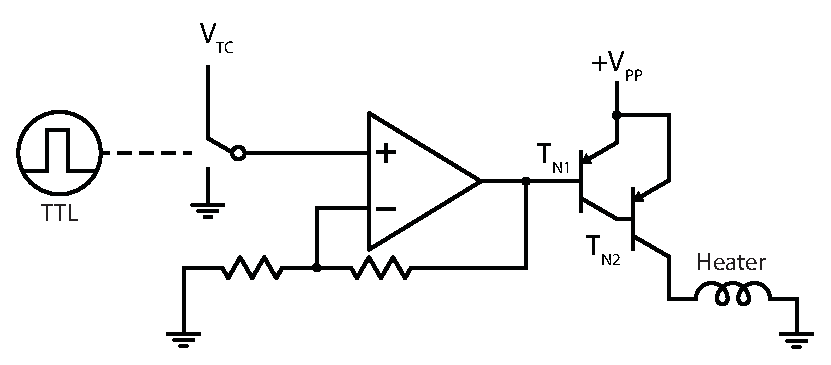
\includegraphics[width=0.8\tw]{figures/magnetometer/HeaterCircuitDC.eps}
\caption{The TTL-controlled DC version of the cell heating circuitry.}
\label{fig:DCHeaterCircuit}
\end{figure}

The input to the op-amp is modulated by a TTL, so that the current can be interrupted during acquisition. This is achieved using a TTL-controlled single-pole double-throw (SPDT) switch, with the ``normally closed'' connection connected to the temperature controller output (V$_{TC}$), and the ``normally open'' connection connected to ground. Because the temperature controller modulates its output to maintain the temperature of the cell at the set temperature, it is preferable for the ``no signal'' mode to revert the circuit to the temperature controller, rather than simply turning the current off. Configurations using a single-pole single-throw (SPST) configuration were insufficient because they left the input to the amplification stage floating, making it subject to various sources of noise. What leakage current and noise remains in the ``grounded'' state typically is filtered out by the Darlington Pair's diode drop, which imposes a voltage threshold condition on amplified current.

\subsubsection{Intermittent cooling}
\label{mag.design.cooling}
The fact that the cell cools over the course of an experiment is a major hindrance to the use of pulsed DC heating, as the temperature of the cell has many direct effects on the signal. According to Newton's law of cooling, the rate of cooling is proportional to the difference in temperature. More precisely\citep{Burmeister1993}

\begin{equation}
\label{eqn:NewtonsLawOfCooling}
\frac{\mathrm{d}Q}{\mathrm{d}t} = hA\Delta T(t),
\end{equation}

where $Q$ (\unit{W}) is the thermal energy, $h$ (\unitfrac{W}{m$^{2}$K}) is the heat transfer coefficient, $A$ (\unit{m$^2$}) is the surface contact area and $\Delta T$ (\unit{K}) is the difference in temperature between the cooling object and the environment. The identity $C = \sfrac{\mathrm{d}Q}{\mathrm{d}t}$ can be substituted into Eqn. \ref{eqn:NewtonsLawOfCooling} to give an equation for the temperature change as a function of time:

\begin{equation}
\label{eqn:TemperatureDifferentialEquation}
\frac{\mathrm{d}T(t)}{\mathrm{d}t} = -\frac{hA}{C}\Delta T(t);
\end{equation}

and the solution to the differential equation is

\begin{equation}
\Delta T(t) = \Delta T_{0}e^{-\sfrac{hAt}{C}}.
\label{eqn:TemperatureLossEquation}
\end{equation}

As this is an exponential decay, most of the heat will be lost in the first part of the decay and so particular care would need to be taken with insulation to avoid any significant temperature drop at the cell. Unfortunately, because of the need for optical access, the cells are likely to be among the least insulated part of the heating apparatus, and because the sample needs to be kept relatively cool but also very close to the cell, it is likely to be near an actively cooled region - leading to a significant temperature gradient (high $\Delta T$). It is also the only part of the magnetometer which needs to be kept warm, as the main downside of cooling is its effect on signal strength.

\subsection{AC Heating}
\label{mag.design.AC.heating}
To avoid some of the problems described in the previous section, the heater was switched from DC to AC - this allows the heater to be operated continuously, so long as the circuit is driven at a frequency far outside the signal bandwidth. This removes the concern about intermittent heating, but leaves open the possibility of parasitic signals.

The AC signal was generated using a Wein bridge oscillator set to \unit[15]{kHz}, output to a \unit[40]{W} audio amplifier; the second amplification step was necessary because AC power is proportional the root-mean-squared value of the voltage and such requires a higher peak-to-peak voltage to apply the same power. Because the magnetometer was configured primarily for low-frequency (<\unit[1]{kHz}) signals, the frequency was chosen to be on the high end of the amplifier bandwidth, around $\approx$ \unit[14]{kHz}.

% \section{Sensitivity Measurement}
% \label{mag.design.sensitivity}
% At least three methods were used to calibrate the sensitivity of the instrument, all of which gave similar but different results. In all of these methods, a specified test signal is applied across the \textit{z} shimming coil and the magnetometer response is measured. The magnetic field response of these coils was calculated from simulations, but if necessary could be measured experimentally using the NMR signal from the sample - since the gyromagnetic ratio of hydrogen is known to high-precision, the magnetic field can be calculated quite accurately from their oscillation frequency.

% The least accurate but quickest method for measuring the sensitivity is to use a lock-in amplifier to modulate the \textit{z} coil and feed the magnetometer signal into the lock-in feedback input\needfact{What is a lock-in feedback input called?}, taking the ratio of the signal and noise channels (both at the carrier frequency)\needfact{What are the right terms for the signal and noise channels here?}. Alternately, the time-domain magnetometer signal can be captured and fourier-transformed (either using the data acquisition console or a spectrum analyzer), and the signal peak compared to the standard deviation of either the signal or the baseline.
\end{document}